\documentclass[11pt]{report}

\usepackage{sectsty}
\usepackage{graphicx}
\usepackage{pdfpages}
\usepackage{etoolbox}
\usepackage{hyperref}
\usepackage[backend=biber,style=numeric,sorting=custom,minnames=3, maxnames=6]{biblatex}
\usepackage{minitoc}
\usepackage{fancyhdr}
\usepackage{longtable}
\usepackage{pdflscape}
\usepackage{varwidth}
\usepackage{amsmath}
\usepackage{bm}
\usepackage{multirow}
\usepackage{parnotes}
\usepackage{booktabs}
\usepackage{xspace}
\usepackage{array}
\usepackage{pifont}
\usepackage{subcaption}
\usepackage{colortbl}
% \usepackage[T1]{fontenc}
% \usepackage[french]{babel}
% \hyphenation{é-chan-tillon-nage}
\usepackage{xcolor}

\definecolor{darkWhite}{rgb}{0.96,0.96,0.96}
\definecolor{bluekeywords}{rgb}{0.13,0.13,1}
\definecolor{greencomments}{rgb}{0,0.5,0}
\definecolor{redstrings}{rgb}{0.9,0,0}

\definecolor{Comment}{RGB}{97,161,176}

\definecolor{btfGreen}{RGB}{51,160,44}
\definecolor{btfRed}{RGB}{190,60,90}

\definecolor{bleuUni}{RGB}{0, 157, 224}
\definecolor{marronUni}{RGB}{68, 58, 49}

\definecolor{bluecite}{HTML}{009DE0}

\definecolor{Paired_1}{RGB}{31,120,180}
\definecolor{Paired_2}{RGB}{166,206,227}
\definecolor{Paired_3}{RGB}{51,160,44}
\definecolor{Paired_4}{RGB}{178,223,138}
\definecolor{Paired_5}{RGB}{227,26,28}
\definecolor{Paired_6}{RGB}{251,154,153}
\definecolor{Paired_7}{RGB}{255,127,0}
\definecolor{Paired_8}{RGB}{253,191,111}
\definecolor{Paired_9}{RGB}{106,61,154}
\definecolor{Paired_10}{RGB}{202,178,214}
\definecolor{Paired_11}{RGB}{177,89,40}
\definecolor{Paired_12}{RGB}{255,255,153}
\definecolor{Accent_1}{RGB}{127,201,127}
\definecolor{Accent_2}{RGB}{190,174,212}
\definecolor{Accent_3}{RGB}{253,192,134}
\definecolor{Accent_4}{RGB}{255,255,153}
\definecolor{Accent_5}{RGB}{56,108,176}
\definecolor{Accent_6}{RGB}{240,2,127}
\definecolor{Accent_7}{RGB}{191,91,23}
\definecolor{Accent_8}{RGB}{102,102,102}
\definecolor{Spectral_1}{RGB}{158,1,66}
\definecolor{Spectral_2}{RGB}{213,62,79}
\definecolor{Spectral_3}{RGB}{244,109,67}
\definecolor{Spectral_4}{RGB}{253,174,97}
\definecolor{Spectral_5}{RGB}{254,224,139}
\definecolor{Spectral_6}{RGB}{255,255,191}
\definecolor{Spectral_7}{RGB}{230,245,152}
\definecolor{Spectral_8}{RGB}{171,221,164}
\definecolor{Spectral_9}{RGB}{102,194,165}
\definecolor{Spectral_10}{RGB}{50,136,189}
\definecolor{Spectral_11}{RGB}{94,79,162}
\definecolor{Set1_1}{RGB}{228,26,28}
\definecolor{Set1_2}{RGB}{55,126,184}
\definecolor{Set1_3}{RGB}{77,175,74}
\definecolor{Set1_4}{RGB}{152,78,163}
\definecolor{Set1_5}{RGB}{255,127,0}
\definecolor{Set1_6}{RGB}{255,255,51}
\definecolor{Set1_7}{RGB}{166,86,40}
\definecolor{Set1_8}{RGB}{247,129,191}
\definecolor{Set1_9}{RGB}{153,153,153}
\definecolor{Set1_10}{RGB}{0,0,0}
\definecolor{Set2_1}{RGB}{102,194,165}
\definecolor{Set2_2}{RGB}{252,141,98}
\definecolor{Set2_3}{RGB}{141,160,203}
\definecolor{Set2_4}{RGB}{231,138,195}
\definecolor{Set2_5}{RGB}{166,216,84}
\definecolor{Set2_6}{RGB}{255,217,47}
\definecolor{Set2_7}{RGB}{229,196,148}
\definecolor{Set2_8}{RGB}{179,179,179}
\definecolor{Dark2_1}{RGB}{27,158,119}
\definecolor{Dark2_2}{RGB}{217,95,2}
\definecolor{Dark2_3}{RGB}{117,112,179}
\definecolor{Dark2_4}{RGB}{231,41,138}
\definecolor{Dark2_5}{RGB}{102,166,30}
\definecolor{Dark2_6}{RGB}{230,171,2}
\definecolor{Dark2_7}{RGB}{166,118,29}
\definecolor{Dark2_8}{RGB}{102,102,102}
\definecolor{Reds_1}{RGB}{255,245,240}
\definecolor{Reds_2}{RGB}{254,224,210}
\definecolor{Reds_3}{RGB}{252,187,161}
\definecolor{Reds_4}{RGB}{252,146,114}
\definecolor{Reds_5}{RGB}{251,106,74}
\definecolor{Reds_6}{RGB}{239,59,44}
\definecolor{Reds_7}{RGB}{203,24,29}
\definecolor{Reds_8}{RGB}{165,15,21}
\definecolor{Reds_9}{RGB}{103,0,13}
\definecolor{Greens_1}{RGB}{247,252,245}
\definecolor{Greens_2}{RGB}{229,245,224}
\definecolor{Greens_3}{RGB}{199,233,192}
\definecolor{Greens_4}{RGB}{161,217,155}
\definecolor{Greens_5}{RGB}{116,196,118}
\definecolor{Greens_6}{RGB}{65,171,93}
\definecolor{Greens_7}{RGB}{35,139,69}
\definecolor{Greens_8}{RGB}{0,109,44}
\definecolor{Greens_9}{RGB}{0,68,27}
\definecolor{Blues_1}{RGB}{247,251,255}
\definecolor{Blues_2}{RGB}{222,235,247}
\definecolor{Blues_3}{RGB}{198,219,239}
\definecolor{Blues_4}{RGB}{158,202,225}
\definecolor{Blues_5}{RGB}{107,174,214}
\definecolor{Blues_6}{RGB}{66,146,198}
\definecolor{Blues_7}{RGB}{33,113,181}
\definecolor{Blues_8}{RGB}{8,81,156}
\definecolor{Blues_9}{RGB}{8,48,107}


\newcommand{\AFFECT}{AFF3CT\xspace}
\newcommand{\Cxx}{\texttt{C++}\xspace}
\newcommand{\cmark}{\textcolor{btfGreen}{\large\ding{51}}}
\newcommand{\xmark}{\textcolor{btfRed}{\footnotesize\ding{55}}}

\newcolumntype{L}[1]{>{\raggedright\let\newline\\\arraybackslash\hspace{0pt}}m{#1}}
\newcolumntype{C}[1]{>{\centering\let\newline\\\arraybackslash\hspace{0pt}}m{#1}}
\newcolumntype{R}[1]{>{\raggedleft\let\newline\\\arraybackslash\hspace{0pt}}m{#1}}
\newlength{\simcolwidth}
\setlength{\simcolwidth}{0.5cm}

% Margins
\topmargin=-0.45in
\evensidemargin=0in
\oddsidemargin=0in
\textwidth=6.5in
\textheight=9.0in
\headsep=0.25in

\title{Habilitation à Diriger des Recherches}
\author{ Mathieu Léonardon }
\date{\today}

\setcounter{secnumdepth}{3}

% Mettre en pied de page le numéro de page comme ailleurs
\fancypagestyle{includepdfstyle}{
  \fancyhf{}
  \fancyfoot[C]{\thepage}
  \renewcommand{\headrulewidth}{0pt} % Remove top rule
  \renewcommand{\footrulewidth}{0pt} % Remove bottom rule
}

\addbibresource{all.bib}

\DeclareSortingTemplate{custom}{
  \sort{
    \field{sortkey}
  }
}

\begin{document}


% Doctoral school
\vspace*{0cm}
\begin{center}
    \Large{\textbf{Université de Bretagne Occidentale}} \\[0.5cm]
    \Large{\textbf{Ecole Doctorale MATHSTIC}} \\[0.1cm]
    \large{\textit{Sciences et Technologies de l'Information et de la Communication}}
\end{center}

% Diploma
\vfill
\begin{center}
    \Huge{\textbf{Habilitation à Diriger des Recherches}}
\end{center}

% Me
\vfill
\begin{center}
    \large{Soutenue par :} \\[0.1cm]
    \Large{\textbf{Mathieu \textsc{Léonardon}}}
\end{center}

% Title
\vfill
\begin{center}
        \centering
        \Huge{\textbf{\textsc{Digital Communication and Deep Learning on Embedded Systems}}} \\[0.5cm]
\end{center}

% Date
\vspace*{0.5cm}
\begin{center}
    \large{Soutenue publiquement le~~~~devant le jury composé de :}
\end{center}

% Jury
\vfill
\begin{center}
    \begin{varwidth}[t]{\maxdimen}
        \begin{center}
            \large{\textit{Rapporteurs}}
        \end{center}
        \large{\textbf{Rapporteur 1}}, Professeur, XXX \\[0.1cm]
        \large{\textbf{Rapporteur 2}}, Professeur, XXX \\[0.1cm]
        \large{\textbf{Rapporteur 3}}, Professeur, XXX
    \end{varwidth}
    \hspace{2cm}
    \begin{varwidth}[t]{\maxdimen}
        \begin{center}
            \large{\textit{Examinateurs}}
        \end{center}
        \large{\textbf{Examinateur 1}}, Professeur, XXX \\[0.1cm]
        \large{\textbf{Examinateur 2}}, Professeur, XXX
    \end{varwidth}
\end{center}


\dominitoc % Active les mini-tables des matières

\tableofcontents
\vspace{1.5cm}


% Logos
% \vspace*{2.2cm}
% \includegraphics[height=1cm]{covers/figures/logo_UBO.png}
% \hfill
% \includegraphics[height=1cm]{covers/figures/logo_MATHSTIC.png}
% \hfill
% \includegraphics[height=1cm]{covers/figures/logo_LABSTICC.png}
% \hfill
% \includegraphics[height=1cm]{covers/figures/logo_IMT.png}

\chapter{Foreword}
The common thread in my work is the simplification of algorithms and efficient implementation, which leads to the principle: you can do just as well with less. The richness of the work primarily comes from the interaction between experts in specific algorithmic fields, mainly channel coding and deep learning, with someone who is concerned with computational and memory economy.

This is what truly motivates me in my research. There is a real pleasure in discovering a new problem and its solutions, and then in a second phase, reflecting with a partner on what can be removed, simplified, factored, and streamlined. It's a celebration of sobriety. One could, lacking humility, claim a consistently positive impact from the perspective of the energy consumption of digital systems and their overall carbon footprint. However, the savings achieved are actually used to perform more processing and to deploy them wherever possible. These issues are more economic and political in nature than scientific.

What motivates me more is the intrinsic challenge of each problem. How far can we go? What is the real impact of the choices we make? I am very fond of competitions in the academic environment, whether in a research or teaching context. Not for the competition itself (though, I must admit, it's in my nature), but mainly because it allows for the definition of an objective criterion and clear procedures to fairly compare implementations.

During this past decade spent in the research world, it is tiring to see published works that are inapplicable but well-marketed. Confronting research ideas with an objective criterion helps to avoid this kind of drift. I have developed competitive aspects in two courses I teach at IMT Atlantique, which I detail in the Appendix~\ref{sec:spotlight_courses}. Competition can also consist of choosing a set of constraints to restrict a more complex problem and then optimizing a metric. This is what I did in my thesis on the implementation of error-correcting codes on general-purpose processors. It is what I pushed Hugo Tessier to do in his thesis on neural network pruning. It is also what I proposed to Hugo Le Blévec in his thesis on the implementation of neural networks for semantic segmentation on FPGAs. Or with a group of students on the Open Hardware competition organized by AMD/Xilinx. Finally, during the implementation competition at the ISTC 2025 conference.

These works and experiences consistently allow for the acquisition of experience and certainties about the methods that do or do not have a strong impact on the performance and efficiency of systems. It is an empirical knowledge that is built over the course of projects and collaborations, and which industrialists are very keen on.

However, while it is necessary to compare ourselves on objective, measurable criteria within controlled frameworks, I am of the opinion that my research activities have focused a little too much on this type of contribution, to the detriment of a more long-term vision aimed at a positive impact on society. The objective of this document is, after summarizing my past activities, to propose perspectives that allow for the application of the knowledge acquired toward a more ambitious goal than winning a competition or being state-of-the-art on a benchmark.
\pagebreak

\chapter{Summary of Research, Supervision, and Funding Activities}
\minitoc
\vspace{1cm}

This chapter summarizes my research activities. I completed a doctoral thesis titled \textit{Decoding of Polar Codes on Programmable Architectures}. These works, continued during a temporary lecturer position (ATER), also led to the creation of open-source software for simulating complete digital communication chains and their implementation in software-defined radio (SDR). This line of research is detailed in Section~\ref{sec:chaines_communication}.
I then reoriented my research towards the compression of deep learning algorithms and their deployment on embedded targets: FPGAs, embedded processors and microcontrollers, and embedded GPUs. Section~\ref{sec:deep_learning_embedded} presents the main contributions in this area.


\section{Digital Communication Algorithms on Programmable Architectures}
\label{sec:chaines_communication}


Software implementations of error-correcting code decoders play a crucial role in several areas of modern digital communications. Firstly, they are essential for Monte Carlo simulations, enabling the evaluation of communication system performance under various noise and interference scenarios. Secondly, in the context of Cloud-RAN (Cloud Radio Access Networks), software decoders offer the flexibility needed to virtualize physical layer functions, thereby facilitating cooperative multi-point processing. These decoders are indeed the most computationally intensive building blocks of the communication chain. Finally, for software-defined radios (SDR), they allow dynamic reconfiguration of communication parameters, adapting systems to different standards and channel conditions without requiring hardware modifications.

My PhD thesis presents efficient implementation methods (throughput, latency, energy consumption) for polar code decoding algorithms on specific hardware architectures (ASIP: Application Specific Instruction-set Processor) but also on general-purpose processors (GPP: General Purpose Processor). This work, in collaboration with Adrien Cassagne from LIP6, led to the creation of the open-source software AFF3CT, a complete software toolbox for the simulation and implementation of digital communication chains.

\subsection{Decoding of Polar Codes on General Purpose Processors}
\label{sec:decoding_polar_codes_gpp}

In the present manuscript, I will focus the discussion on my key contributions in the field of polar code decoding. I will therefore skip everything concerning code construction and decoding techniques that fall outside the scope of my contributions. I invite the reader to refer to my PhD manuscript for these topics \cite{leonardon:tel-01997553}. I will, however, attempt to clearly explain the structure of the SCL and SCAN decoding algorithms, their scheduling, and their potential for parallelization using diagrams. I will also describe their refinements (FAST-SCL and Adaptive simplification) in Section~\ref{sec:sc_list_scan} before clearly presenting the contributions I proposed and the results obtained in Section~\ref{sec:fast_flexible_polar_decoders}. More recent developments and new results, obtained during my participation in the ISTC 2025 (International Symposium on Topics in Coding) conference, are presented in Section~\ref{sec:istc25_challenge}.

\subsubsection{SC-List and SCAN decoding algorithms}
\label{sec:sc_list_scan}

Polar codes, introduced by Arıkan in 2009, are the first error-correcting codes proven to achieve Shannon capacity for infinite code lengths~\cite{Arikan2009}. The Successive Cancellation (SC) decoding algorithm was initially proposed for polar codes, but its performance in terms of bit error rate (BER) and frame error rate (FER) is insufficient for short code lengths. To address this, the Successive Cancellation List (SCL) algorithm was proposed in the literature, significantly improving decoding performance by maintaining a list of candidate paths. An optimized version, called Fast SCL, was subsequently developed to reduce computational complexity while maintaining good decoding performance. These algorithms allow for trade-offs between complexity, latency, and decoding performance, making polar codes suitable for modern communication standards like 5G.

The polarization phenomenon and polar codes were developed assuming the use of the Successive Cancellation (SC) decoding algorithm. This is a hard-output algorithm, meaning the output data consists of bits. However, a second decoding algorithm, Belief Propagation (BP), was also proposed. This one is a soft-output algorithm. This means that the output data are estimates typically represented as LLRs (Log-Likelihood Ratios). As a reminder, in the LLR representation, the sign corresponds to the hard decision: a bit equal to 0 for a positive LLR, and a bit equal to 1 for a negative LLR. The absolute value indicates the reliability of this decision.

Although the SC algorithm is asymptotically optimal as N tends to infinity, its performance is limited for finite-sized codes. Numerous variants of these algorithms have therefore been proposed to improve their error correction performance. The Successive Cancellation List (SCL) algorithm is an evolution of the SC algorithm. Furthermore, the algorithm called Soft Cancellation (SCAN) can be seen as a combination of the SC and BP algorithms. Each of these algorithms is described in this section.

\begin{figure}[t]
\centering
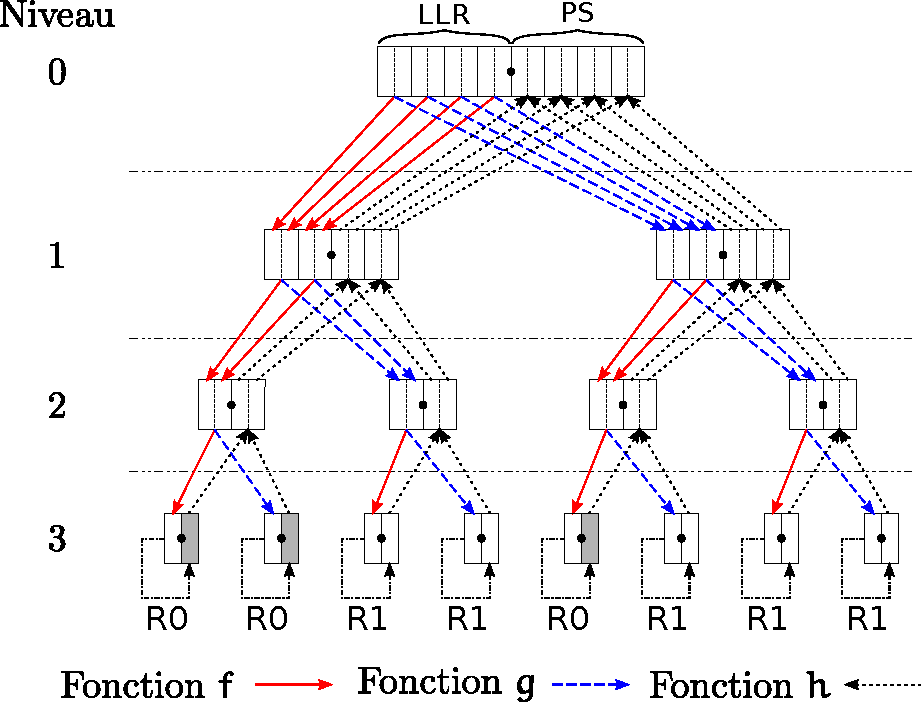
\includegraphics[width=0.55\textwidth]{fig/sc}
\caption{SC decoding tree.}
\label{fig:sc}
\end{figure}


\begin{eqnarray}
  \begin{array}{l c l}
    f(L_a,L_b) &=& \text{sign}(L_a.L_b).\min(|L_a|,|L_b|)\\
    g(L_a,L_b,\hat{s}_a)&=&(1-2\hat{s}_a)L_a+L_b\\
    h(\hat{s}_a,\hat{s}_b)&=& (\hat{s}_{a} \oplus \hat{s}_{b}, \hat{s}_{b})\\
    \texttt{R0}(L_a) &=& 0 \\
    \texttt{R1}(L_a) &=&  \left\{\begin{array}{l c l} 0 \text{ si } L_a \geq 0 \\ 1 \text{ si } L_a < 0 \end{array}\right.
  \end{array}
  \label{eq:sc}
\end{eqnarray}
\paragraph{Successive Cancellation} decoding can be represented as a traversal of a binary tree. The tree representation, as shown in Figure~\ref{fig:sc}, is an alternative representation that highlights certain algorithmic simplifications.
The data are organized in a binary tree with $log_2(N) + 1$ \textbf{levels}. In our pedagogical example, the tree has four levels.
At each level, a certain number of \textbf{nodes} are assigned.
The \textbf{root} of the tree, numbered $0$, consists of a single node.
The root contains $N$ LLRs and $N$ partial sums.
As the tree is traversed, at each level, the number of nodes doubles.
Conversely, the number of LLRs and partial sums in each node is halved.
The \textbf{leaves} are the nodes of the last level of the tree (level 3 in Figure~\ref{fig:sc}).
Processing a leaf corresponds to applying the \texttt{R0} and \texttt{R1} operations.
Each level $d$ contains $2^d$ nodes, each consisting of $2^{n-d}$ LLRs and $2^{n-d}$ partial sums, where $n=\log_2(N)$.
The partial sums are propagated by the function $h$. They are propagated up to a level that depends on the index of the leaf that has just been processed.
In the case of a non-systematic polar code, the decoded sequence $\hat{u}$ is composed of the partial sums contained in the leaves of the decoding tree.
During non-systematic decoding, the partial sums contained in the leaves correspond to the decoded sequence $\hat{u}$.

Figure~\ref{fig:seq_sc} is a more compact representation of the decoding tree.
Operations 12 and 13 in Figure~\ref{fig:seq_sc} are therefore redundant since they only serve to compute the partial sums of the root node.
In the case of a systematic code, it is the partial sums of the root node that correspond to the decoded codeword.
The traversal of the tree is a depth-first traversal.
The scheduling of the different functions is detailed in Figure~\ref{fig:seq_sc}, where each arrow representing a function is numbered according to the execution order.

\begin{figure}[t]
\centering
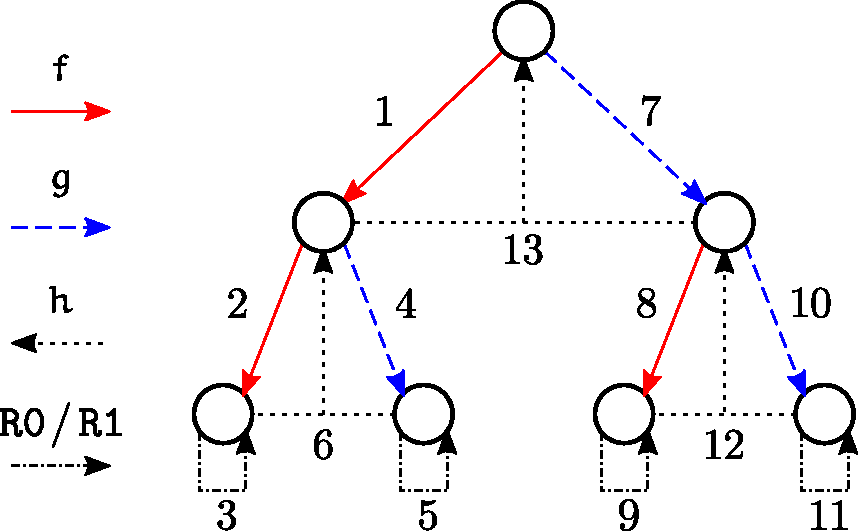
\includegraphics[width=0.5\textwidth]{fig/seq_sc}
\caption{Scheduling of SC decoding for a polar code of size $N=4$.}
\label{fig:seq_sc}
\end{figure}

\paragraph{Successive Cancellation List} (SCL) decoding algorithm is an extension of the SC algorithm~\cite{Tal2015}. The SC algorithm suffers from limited error-correction performance for short and moderate-length polar codes ($N < 8192$), whereas SCL decoding significantly improves these results.

\begin{figure}[t]
\centering
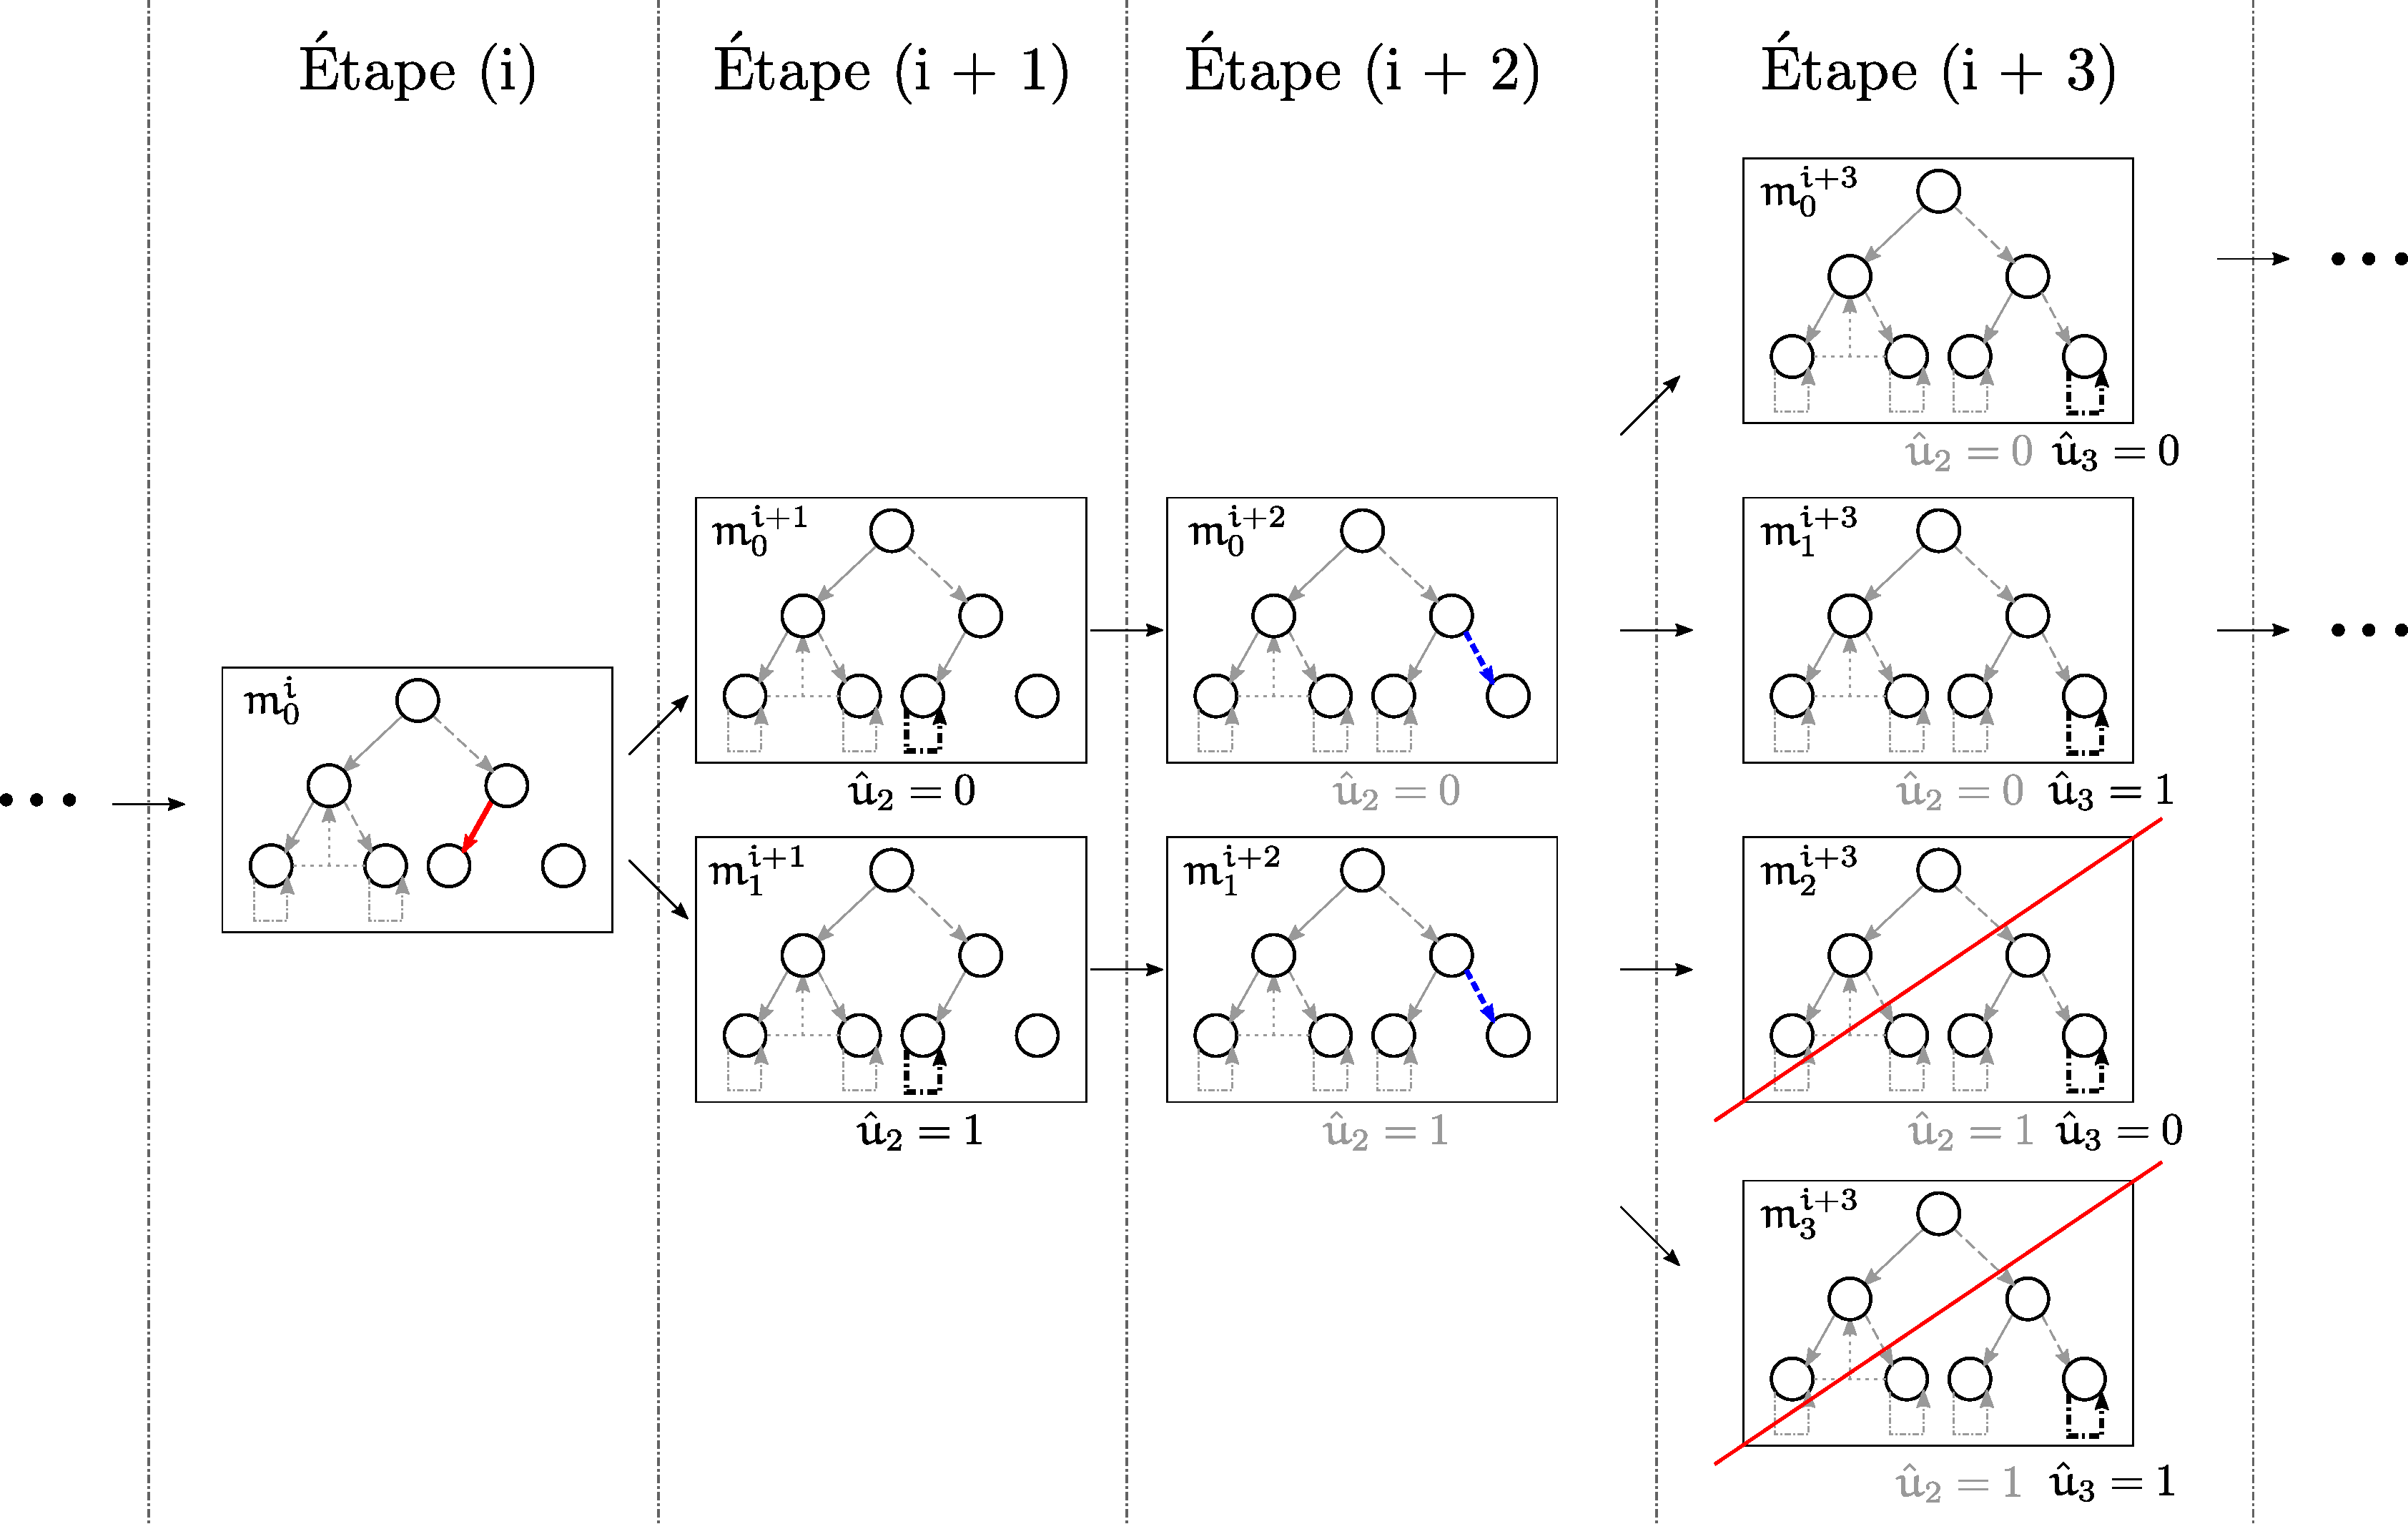
\includegraphics[width=1\textwidth]{fig/scl}
\caption{Duplication de l'arbre de décodage dans l'algorithme SCL.}
\label{fig:scl}
\end{figure}

In the previously described SC decoder, hard decisions are applied whenever a leaf corresponding to an information bit is processed (operation \texttt{R1}). If an error is made at this stage, it cannot be corrected, and the decoding of the codeword fails. The key idea of list decoding is to postpone hard decisions. Instead of applying a threshold directly to the LLR, both possible decoding outcomes are explored. To do so, the decoding tree, together with all its LLRs and partial sums, is duplicated. This process is illustrated in Figure~\ref{fig:scl}.

The algorithm is shown at step (i), where the function $f$ is applied. At the next step (i+1), the decoding tree is duplicated to create two paths: one assuming $\hat{u}_2=0$, and the other assuming $\hat{u}_2=1$. Decoding then proceeds in parallel along both paths. At step (i+2), the function $g$ is applied. These two trees are referred to as decoding \textbf{paths}. At each leaf of rate 1, the same procedure is applied, doubling the number of paths to be decoded in parallel, as shown at step (i+3).

\paragraph{Concatenation with a CRC}

The authors of~\cite{Tal2015} proposed concatenating a Cyclic Redundancy Check (CRC) to discriminate between the different candidates. The corresponding encoding is illustrated in Figure~\ref{fig:crc}. A CRC is an error-detecting code. It associates with any binary sequence, here $\bm{b}$ of length $K$, a sequence of length $K+c$. After decoding, the CRC verification allows the detection of potential errors. The CRC is designed so that the probability of an undetected error is extremely small.
Thus, at the end of the decoding algorithm, when the $\mathrm{L}$ candidate codewords at the output of the SCL algorithm are available, a CRC verification is performed. If one of them passes the CRC check, it is then highly probable that it is the correct candidate. In the rare case where several candidates pass the CRC check, the one with the smallest metric among them is selected. When this candidate selection mechanism based on CRC verification is applied, the algorithm is referred to as CRC-Aided SCL (CASCL).

\begin{figure}[t]
\centering
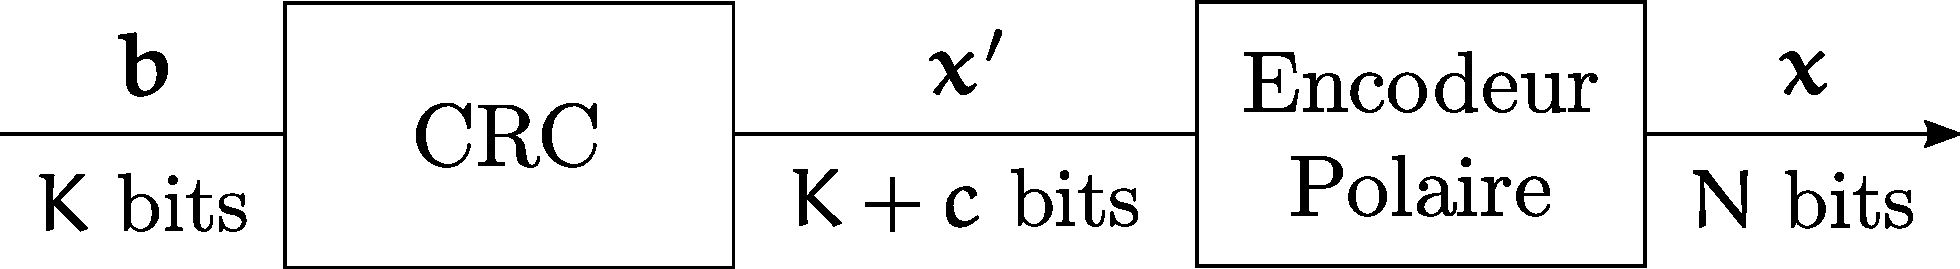
\includegraphics[width=0.6\textwidth]{fig/crc}
\caption{Concatenation with a CRC.}
\label{fig:crc}
\end{figure}

\paragraph{Adaptive SCL Decoding Algorithms}
\label{subsubsec:adaptive}

The CASCL algorithm significantly improves decoding performance compared to the SC algorithm.
However, this improvement comes at the cost of increased computational complexity.
Nevertheless, it is possible to combine the two algorithms, SC and CASCL, in order to approach the low computational complexity of the former while preserving the decoding performance of the latter~\cite{Li2012}.
The principle is as follows: a first decoding attempt is performed with the SC algorithm. The CASCL algorithm is then triggered only if a decoding error is detected through CRC verification.

Two variants of the adaptive algorithm are possible.
In the case of the Partially Adaptive SCL (PASCL) algorithm presented in~\cite{Sarkis2016}, when SC decoding fails, the CASCL algorithm is executed only once with a list size of $\mathrm{L}_{max}$.
In the case of the Fully Adaptive SCL (FASCL) algorithm originally proposed in~\cite{Li2012}, the CASCL algorithm may be applied several times. The first CASCL decoding attempt is performed with $\mathrm{L}=2$. If, after decoding, the CRC is still not satisfied, the algorithm is relaunched as many times as necessary, iteratively doubling $\mathrm{L}$ until reaching $\mathrm{L}_{max}$.


\paragraph{Pruning of the polar decoding tree}
To reduce the computational complexity of the SC decoding algorithm, the decoding tree can be pruned as described in~\cite{Alamdar-Yazdi2011}. For instance, a subtree whose leaves are all rate-0 (frozen bits) does not need to be traversed, since all its partial sums are necessarily zero. Similarly, a subtree whose leaves are all rate-1 can be replaced by directly applying the thresholding function \texttt{R1} at its root, which yields the same result as a full traversal.

Beyond these two simple cases, other subtree patterns have also been identified, such as repetition (\texttt{REP}) and single parity check (\texttt{SPC}) nodes~\cite{Sarkis2014a}. For these structures, dedicated decoding techniques can be applied to derive the partial sums directly from the LLRs at the root, again avoiding traversal of the entire subtree.

The advantage of such pruning, often referred to as Fast-SC, is a drastic reduction of both computational and control complexity, which is especially relevant for software implementations where tree traversal is costly. Importantly, these techniques are not limited to SC decoding: they can be extended to list decoding as well, leading to the Fast-SCL algorithm~\cite{Sarkis2016}. The complexity reduction becomes particularly significant when the code rate is close to 0 or close to 1.

\begin{figure}[h]
  \centering
  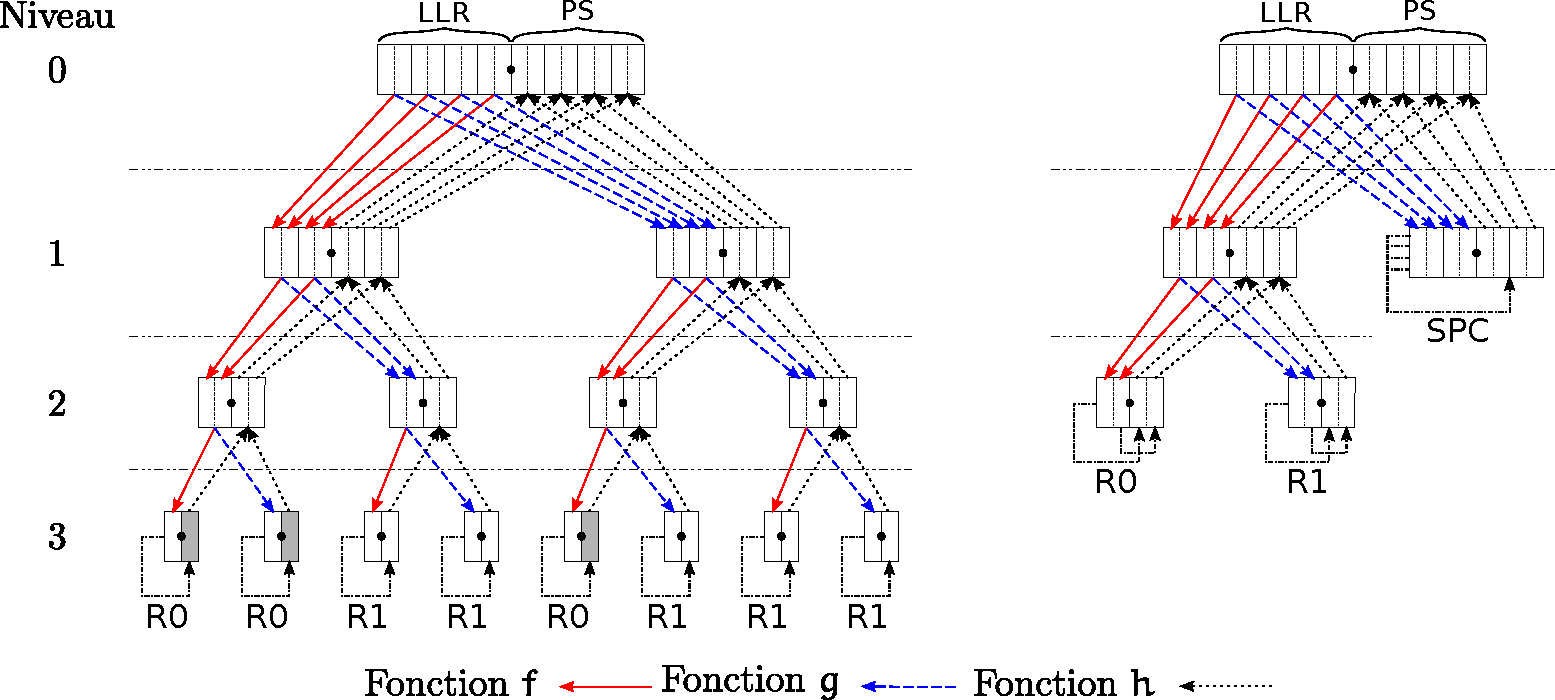
\includegraphics[width=\textwidth]{fig/sc_tree_pruned.pdf}
  \caption{Pruning of the SC decoding tree.}
  \label{fig:sc_pruned}
\end{figure}

\subsubsection{A Fast and Flexible Software Implementation of Polar Code Decoders}
\label{sec:fast_flexible_polar_decoders}

Software implementation of channel codes has emerged as a compelling alternative to dedicated hardware. It enables rapid prototyping and validation of new algorithms, while offering high flexibility to support a wide variety of codes and decoding strategies. Unlike hardware, software decoders can be easily configured to trade off correction capability, latency, and throughput, making them well suited for adaptive schemes. They also facilitate reproducibility and portability across platforms. At the network level, software implementations align with the trend toward Cloud-RAN, where virtualized signal processing allows dynamic allocation of resources, improved inter-cell cooperation, reduced energy consumption, and lower communication latency.

The software implementation on General Purpose Processors (GPP) is a complete discipline, and it is not possible to present here the full set of methods, best practices, and techniques required to achieve good latency and throughput performance. Nevertheless, we highlight a few important techniques.

First, vectorization. Every modern GPP includes vector processing units, which are hardware modules within the processor capable of performing several identical computations in parallel on different (but contiguous) data. This is referred to as SIMD – Single Instruction Multiple Data. In polar decoding trees, these instructions are particularly useful to accelerate processing, as they allow several of the previously listed functions to be computed simultaneously when traversing from one node of the tree to another. Vectorization can be applied within a single decoding tree (intra-frame) or by processing several frames in parallel (inter-frame). The first case is more challenging since the number of processed data varies with the depth of the decoding tree. This number may even fall below the size of the vector registers at the lowest nodes, resulting in incomplete utilization of parallelism. In contrast, inter-frame parallelization does not suffer from this limitation, since the number of frames can be chosen to fully occupy the vector registers. However, its drawback lies in frame size: for large codewords, the cache capacity of the processors may be exceeded, leading to a collapse of performance.

A second technique, closely related to vectorization, is data quantization. It is possible to represent data in SC and SCL decoding trees with fewer than 32 bits, typically 16 or 8. This brings two main advantages. First, it increases the parallelism of vector instructions. Second, it reduces the memory footprint of the decoding trees, thereby decreasing cache usage and lowering the memory bandwidth requirements.

Finally, another notable technique is \emph{unrolling}. This consists in explicitly expanding the loops of the decoding algorithm in the source code, instead of relying on iterative loop execution. By doing so, the control overhead associated with loop counters and branching is eliminated, and the compiler can optimize the resulting straight-line code more aggressively. In the context of polar decoders, unrolling allows to reduce the latency of critical functions by removing conditional branches and improving instruction-level parallelism. However, the main drawbacks are, first, the increase in code size, which can become significant for large code lengths, and second, the lack of flexibility: for implementations supporting different code sizes or rates, dedicated source codes would need to be generated, which is not practical.


I proposed several major contributions for the software implementation of SCL decoders~\cite{leonardon:hal-01987848}.

\paragraph{Fine-grained Pruning Configuration}
I allowed fine control over tree pruning in our polar decoder implementations, enabling or disabling different node types (\texttt{R0}, \texttt{R1}, \texttt{REP}, \texttt{SPC}) independently. Figures~\ref{fig:nodes} and~\ref{fig:spc_impact} illustrate how enabling certain nodes affects coded throughput and decoding performance. High-rate codes benefit more from \texttt{R1} pruning, while low-rate codes gain more from \texttt{R0} and \texttt{REP} pruning; \texttt{SPC} nodes show a less clear trend. Allowing \texttt{SPC} nodes larger than 4 (\texttt{SPC4+}) increases throughput by 8–20% but may slightly degrade FER depending on the code and list depth. The pruning is dynamically activated, suggesting potential for a real-time adaptive pruning software decoder.

\begin{figure}[t]
  \centering
  \begin{minipage}{0.48\textwidth}
    \centering
    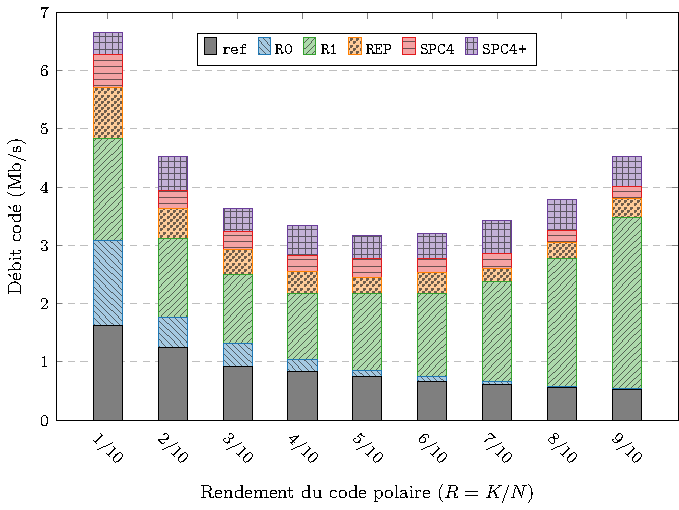
\includegraphics[width=\textwidth]{fig/tree}
    \caption{Impact of activating pruning nodes in the CASCL algorithm, $N=2048$, $\mathrm{L}=32$, $c=32$.}
    \label{fig:nodes}
  \end{minipage}\hfill
  \begin{minipage}{0.48\textwidth}
    \centering
    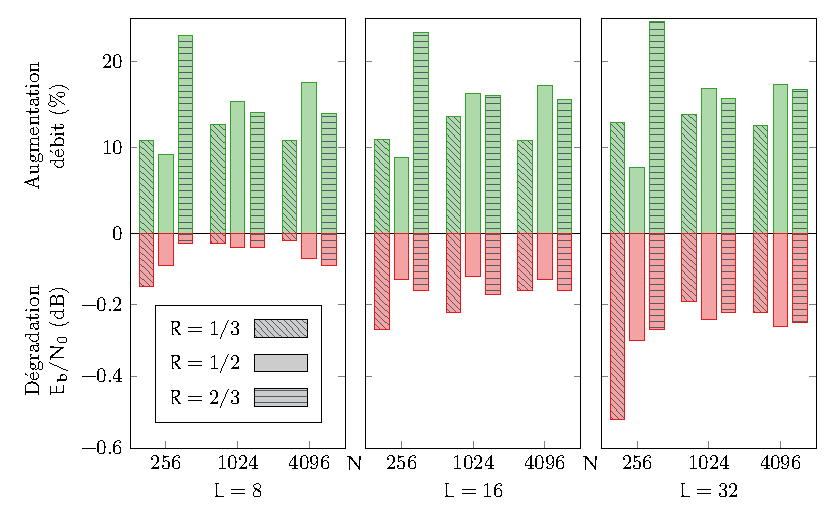
\includegraphics[width=\textwidth]{fig/thr_spc_diff}
    \caption{Effects of using \texttt{SPC4+} nodes in the CASCL algorithm for a FER of $10^{-5}$.}
    \label{fig:spc_impact}
  \end{minipage}
\end{figure}


\paragraph{Fixed-Point Representation}
I implemented SCL decoders using 8- and 16-bit fixed-point representations for LLRs and path metrics to increase parallelism and improve throughput. Figure~\ref{fig:bfer_rep} shows that 16-bit fixed-point representation matches floating-point performance, while 8-bit representation can cause overflow in large repetition nodes (\texttt{REP}). Disabling large repetition nodes (\texttt{REP8-}) eliminates performance loss for 8-bit representation. Table~\ref{tab:quantif} demonstrates that fixed-point representations reduce latency and increase throughput, e.g., FASCL achieves 425.9 Mb/s with 8-bit LLRs. This allows efficient, high-throughput software implementations without significant loss in decoding performance.

\begin{figure}[t]
  \centering
  \begin{minipage}{0.48\textwidth}
    \centering
    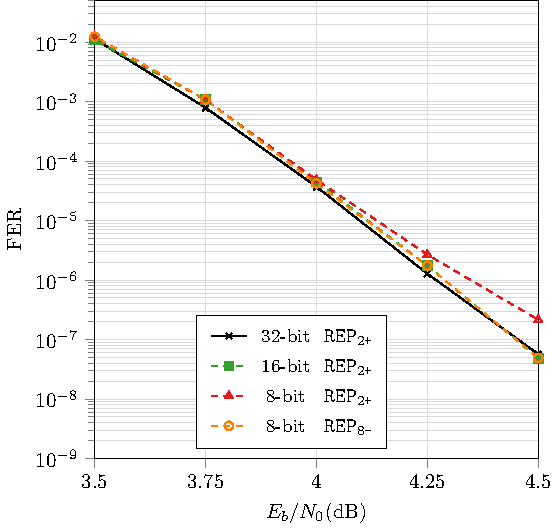
\includegraphics[width=\textwidth]{fig/bfer_rep}
    \caption{Impact of using repetition nodes on quantized implementations.}
    \label{fig:bfer_rep}
  \end{minipage}\hfill
  \begin{minipage}{0.48\textwidth}
    \centering
    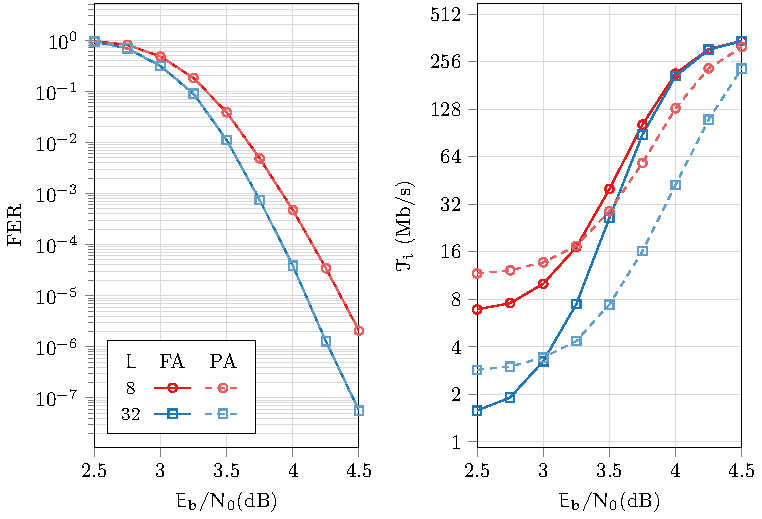
\includegraphics[width=\textwidth]{fig/ascl}
    \caption{Decoding performance and throughput of the PASCL and FASCL decoding algorithms for a polar code ($2048$,$1723$), $\mathrm{L}=32$, and CRC $c=32$ GZip.}
    \label{fig:ascl_perfs}
  \end{minipage}
\end{figure}

  \begin{table}[b]
    \renewcommand{\arraystretch}{1.1}
    \centering
    \caption{Comparaison de débits et latences des algorithmes SCL adaptatifs pour des représentations à virgule flottante (32 bits) et virgule fixe (16 et 8 bits). Code polaire ($2048$,$1723$), $\mathrm{L}=32$, CRC $c=32$ (GZip).}
    \label{tab:quantif}
    {\small\resizebox{0.8\linewidth}{!}{
    \begin{tabular}{r | c | c || c | c || c | c || c | c}
      \multirow{2}{*}{\textbf{Décodeur}} & \multirow{2}{*}{\textbf{Quantif.}} & \multirow{2}{*}{$\bm{\mathcal{L}_{PC}}$} & \multicolumn{2}{c ||}{\textbf{3.5 dB}} & \multicolumn{2}{c ||}{\textbf{4.0 dB}} & \multicolumn{2}{c}{\textbf{4.5 dB}} \\
      \cline{4-9}
      & & & $\bm{\mathcal{L}_{moy}}$ & $\bm{\mathcal{T}_i}$ & $\bm{\mathcal{L}_{moy}}$ & $\bm{\mathcal{T}_i}$ & $\bm{\mathcal{L}_{moy}}$ & $\bm{\mathcal{T}_i}$ \\
      % \hline
      \hline
      \multirow{3}{*}{PA-SSCL} & 32-bit &  635 & 232.3 &   7.6 & 41.7 &  42.1 & 7.4 & 237.6 \\
      %\cline{3-9}
                               & 16-bit &  622 & 219.6 &   8.0 & 40.1 &  43.8 & 6.6 & 267.5 \\
      %\cline{3-9}
                               &  8-bit &  651 & 232.4 &   7.6 & 41.2 &  42.6 & 6.5 & 268.3 \\
      \hline
      \multirow{3}{*}{FA-SSCL} & 32-bit & 1201 &  67.2 &  26.1 &  8.5 & 207.8 & 5.1 & 345.5 \\
      %\cline{3-9}
                               & 16-bit & 1198 &  68.7 &  25.6 &  7.7 & 225.7 & 4.3 & 408.7 \\
      %\cline{3-9}
                               &  8-bit & 1259 &  71.8 &  24.4 &  7.7 & 227.3 & 4.1 & 425.9 \\
    \end{tabular}
    }}
  \end{table}


\begin{figure}
\centering
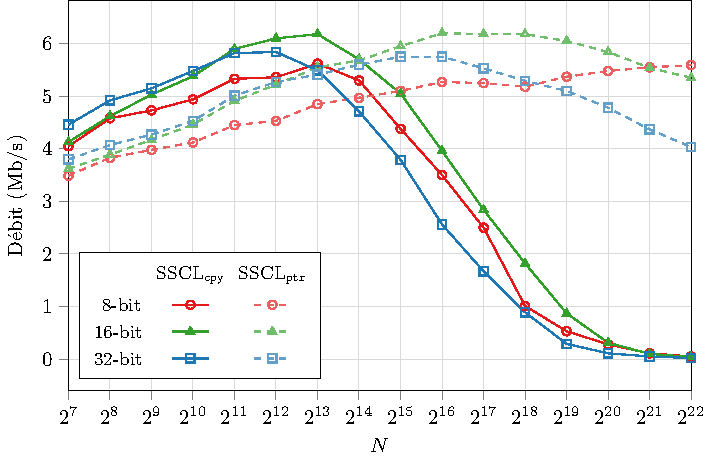
\includegraphics[width=0.6\linewidth]{fig/thr}
\caption{Comparison of throughputs associated with the $SCL_{cpy}$ and $SCL_{ptr}$ methods for different values of $N$.}
\label{fig:scl_mem}
\end{figure}

\begin{table}[hb!]
  \centering
  \caption{Comparison of throughputs and latencies of the proposed decoders with those from the state of the art. LLRs and partial sums represented on 32 bits. Polar code (2048,1723), $\mathrm{L}=32$, CRC GZip $c=32$.}
  \label{tab:res}
  {\small\resizebox{0.8\linewidth}{!}{
  \begin{tabular}{r|l|c|c|c c c}
    \multirow{2}{*}{\textbf{Target}} & \multirow{2}{*}{\textbf{Algorithm}} & \multirow{2}{*}{\textbf{Version}}  & \multirow{1}{*}{\textbf{$\bm{\mathcal{L}_{PC}}$}} & \multicolumn{3}{c}{$\bm{\mathcal{T}_i}$ (Mb/s)} \\
    \cline{5-7}
    &                        &   & ($\mu s$)                          & \textbf{3.5 dB} & \textbf{4.0 dB} & \textbf{4.5 dB} \\
    \hline
    \parnoteclear
    i7-4790K & CASCL \parnote{{\footnotesize Non-pruned version of the CASCL algorithm.}\label{pn:note}}  &~\cite{Shen2016}      & 1572                           & 1.10            & 1.10            & 1.10            \\
    \hline
    i7-2600  & CASCL\textsuperscript{1} &~\cite{Sarkis2014a}     & 23000                          & 0.07            & 0.07            & 0.07            \\
    i7-2600  & CASCL\textsuperscript{1} &~\cite{Sarkis2016}           & 2294                           & 0.76            & 0.76            & 0.76            \\
    i7-2600  & CASCL\textsuperscript{1} & This work                        & 4819                           & 0.37            & 0.37            & 0.37            \\
    i5-6600K & CASCL\textsuperscript{1} & This work                        & 3635                           & 0.48            & 0.48            & 0.48            \\
    \hline
    i7-2600  & CASCL &~\cite{Sarkis2014a}    & 3300                           & 0.52            & 0.52            & 0.52            \\
    i7-2600  & CASCL &~\cite{Sarkis2016}          & 433                            & 4.0             & 4.0             & 4.0             \\
    i7-2600  & CASCL & This work                       & 770                            & 2.3             & 2.3             & 2.3             \\
    i5-6600K & CASCL & This work                       & 577                            & 3.0             & 3.0             & 3.0             \\
    \hline
    i7-2600  & PASCL &~\cite{Sarkis2014a}    & $\approx$ 3300                 & 0.9             & 4.90            & 54.0            \\
    i7-2600  & PASCL &~\cite{Sarkis2016}          & $\approx$ 433                  & 8.6             & 33.0            & 196.0           \\
    i7-2600  & PASCL & This work                       & 847                            & 5.5             & 31.1            & 168.4           \\
    i5-6600K & PASCL & This work                       & 635                            & 7.6             & 42.1            & 237.6           \\
    \hline
    i7-2600  & FASCL & This work                       & 1602                           & 19.4            & 149.0           & 244.3           \\
    i5-6600K & FASCL & This work                       & 1201                           & 26.1            & 207.8           & 345.5           \\
  \end{tabular}
  }}
  \parnotes
\end{table}
\paragraph{Adaptive SCL Algorithm Variants}
Two adaptive SCL algorithms were implemented: Partially Adaptive (PASCL) and Fully Adaptive (FASCL), shown in Figure~\ref{fig:ascl_perfs}. PASCL is faster at low SNRs due to fewer intermediate decodings, while FASCL is superior at intermediate SNRs because it executes the algorithm with multiple intermediate list sizes. At high SNRs, both algorithms achieve similar throughput as SC decoding often suffices. Worst-case latency is higher for FASCL, as verified in Table~\ref{tab:quantif}. These implementations highlight the flexibility of our decoder, including dynamic pruning and support for different list-adaptive strategies.


\paragraph{Partial Sum Management}
We store partial sums in fixed-size integers matching LLR representation to exploit SIMD instructions. Memory footprint is reduced from $\mathrm{L}(2N-1)$ to $\mathrm{L}N$ for SCL by reusing memory when possible. We compare two assignment methods during duplication: copying ($SCL_{cpy}$) and pointer-based ($SCL_{ptr}$). $SCL_{cpy}$ is faster for small and medium codes ($N<8192$), while $SCL_{ptr}$ is more efficient for large codes, especially with 8-bit representation (Figure~\ref{fig:scl_mem}). This optimization reduces memory overhead and improves throughput depending on code size and data representation.

\paragraph{Partial Sorting Algorithm}
A new sorting method based on Schreier's tournament algorithm was proposed to select the smallest LLRs or path metrics during SCL execution~\cite{Schreier1932}. Compared to bubble sort, quick-sort, heap-sort, PSN networks, Schreier's method achieves the fastest execution in all tested scenarios, including \texttt{SPC} nodes. This simplifies the software design by using a single, efficient algorithm for all partial sorting operations. Although PSNs could theoretically improve throughput, we do not implement them due to the complexity of creating generic networks for any list size and pruning configuration.

\paragraph{Accelerated CRC Checking}
Profiling shows that CRC verification consumes significant execution time, as it is performed once per SC decoding and L times per SCL decoding. We accelerate CRC by packing 32 bits together, using precomputed CRC sequences, and exploiting pruning nodes for parallel extraction. For FASCL decoding of a polar code (2048,1723) with CRC-32 at $E_b/N_0=4.5$ dB, throughput increases from 262 Mb/s to 426 Mb/s (63\% gain). This approach reduces the computational complexity of CRC extraction and verification while integrating efficiently with SIMD operations.

\paragraph{Comparison with the State of the Art}
The throughputs and latencies of the proposed implementations are detailed in this section. All reported results were obtained using the AFF3CT tool~\cite{cassagne:hal-02358306}. The source code of this software is open and available online. Therefore, all results are easily reproducible. The hardware target is an Intel i5-6600K CPU with Skylake architecture. The AVX2 SIMD instruction set is exploited. Its frequency for the reported results is 3.9 GHz. Compilation was performed on a Linux OS with the GNU C++ compiler (version 5.4.0). The applied compilation options are: \texttt{-Ofast -march=native -funroll-loops}.



\begin{table}[h]
  \centering
  \caption{Comparison of throughputs, number of clock cycles required to decode one frame, and energy per decoded bit, for the proposed decoders on different hardware targets. Fixed-point representation on 8 bits, $E_b/N_0 = 4.5dB$, CRC GZip $c=32$.}
  \label{tab:port}
  {\small\resizebox{0.8\linewidth}{!}{
  \begin{tabular}{r|c|c|c c c c| c c c| c c c}
    \multirow{3}{*}{\centering \textbf{Target}}  & \multirow{3}{*}{\begin{minipage}{0.5in}\centering \textbf{Freq. (MHz)}\end{minipage}} & \multirow{3}{*}{\centering \textbf{Algo.}}  & & \multicolumn{3}{c|}{$\bm{\mathcal{T}_i}$ \textbf{(Mb/s)}} & \multicolumn{3}{c|}{\textbf{\# Cycles per frame}} & \multicolumn{3}{c}{$\bm{\mathcal{E}_b}$ \textbf{(nJ/bit)}} \\
    \cline{4-13}
     & & & & \textbf{3.5} & \textbf{4.0} & \textbf{4.5} & \textbf{3.5} & \textbf{4.0} & \textbf{4.5} & \textbf{3.5} & \textbf{4.0} & \textbf{4.5} \\
     & & & & \textbf{dB}  & \textbf{dB}  & \textbf{dB}  & \textbf{dB}  & \textbf{dB}  & \textbf{dB}  & \textbf{dB}  & \textbf{dB}  & \textbf{dB}  \\

           \hline
      \hline
      \multirow{3}{*}{\begin{minipage}{0.5in}\centering i7 4790\end{minipage}}     & \multirow{3}{*}{\begin{minipage}{0.5in}\centering 3592\end{minipage}}
        & CASCL &                     &  2.34  & 2.38   & 2.24   & 2645 & 2600 & 2763 & 6325 & 6218 & 6607 \\
      & & PASCL &                     &  5.80  & 33.88  & 207.96 & 1067 & 183  & 30   & 2552 & 437  & 71   \\
      & & FASCL &                     &  19.43 & 194.66 & 372.30 & 319  & 32   & 17   & 762  & 76   & 40   \\

      \hline
      \multirow{3}{*}{\begin{minipage}{0.5in}\centering Ryzen 2700X\end{minipage}} & \multirow{3}{*}{\begin{minipage}{0.5in}\centering 4230\end{minipage}}
        & CASCL &                     &  2.68  & 2.72   & 2.56   & 2675 & 2635 & 2800 & 5149 & 5074 & 5391 \\
      & & PASCL &                     &  6.55  & 38.76  & 237.78 & 1094 & 185  & 30   & 2107 & 356  & 58   \\
      & & FASCL &                     &  20.93 & 209.37 & 406.15 & 342  & 34   & 18   & 659  & 66   & 34   \\

      \hline
      \multirow{3}{*}{\begin{minipage}{0.5in}\centering Cortex A73\end{minipage}} & \multirow{3}{*}{\begin{minipage}{0.5in}\centering 2360\end{minipage}}
        & CASCL &                     &  1.23  & 1.28   & 1.20   & 3310 & 3175 & 3382 & 1475 & 1415 & 1507 \\
      & & PASCL &                     &  3.08  & 18.90  & 100.75 & 1319 & 215  & 40   & 588  & 96   & 18   \\
      & & FASCL &                     &  10.64 & 83.58  & 137.37 & 382  & 49   & 30   & 170  & 22   & 13   \\

      \hline
      \multirow{3}{*}{\begin{minipage}{0.5in}\centering Cortex A15\end{minipage}} & \multirow{3}{*}{\begin{minipage}{0.5in}\centering 2000\end{minipage}}
        & CASCL &                     &  0.74  & 0.74   & 0.70   & 4639 & 4639 & 4923 & 3365 & 3365 & 3571 \\
      & & PASCL &                     &  1.81  & 11.06  & 61.86  & 1899 & 312  & 56   & 1378 & 226  & 40   \\
      & & FASCL &                     &  6.23  & 52.77  & 88.31  & 553  & 65   & 39   & 401  & 47   & 28   \\

      \hline
      \multirow{3}{*}{\begin{minipage}{0.5in}\centering Cortex A53\end{minipage}} & \multirow{3}{*}{\begin{minipage}{0.5in}\centering 1840\end{minipage}}
        & CASCL &                     &  0.48  & 0.48   & 0.45   & 6560 & 6560 & 7064 & 1353 & 1353 & 1457 \\
      & & PASCL &                     &  1.17  & 7.32   & 42.77  & 2701 & 433  & 74   & 557  & 89   & 15   \\
      & & FASCL &                     &  4.45  & 39.70  & 68.32  & 712  & 80   & 46   & 147  & 16   & 10   \\

      \hline
      \multirow{3}{*}{\begin{minipage}{0.5in}\centering Cortex A7\end{minipage}} & \multirow{3}{*}{\begin{minipage}{0.5in}\centering 1400\end{minipage}}
        & CASCL &                     &  0.28  & 0.29   & 0.27   & 8615 & 8318 & 8934 & 1071 & 1034 & 1111 \\
      & & PASCL &                     &  0.71  & 4.26   & 21.89  & 3397 & 566  & 110  & 423  & 70   & 14   \\
      & & FASCL &                     &  2.41  & 19.40  & 30.93  & 1001 & 124  & 78   & 124  & 15   & 10   \\

  \end{tabular}
  }}
\end{table}

Our work demonstrates a significant advantage over fully unrolled decoders from the literature by offering a high degree of flexibility. The proposed implementations are generic and easily portable, allowing the use of quantized representations, configurable puncturing patterns, and adaptive decoding algorithms—features not available in prior works. The throughput and latency results of the proposed decoders are detailed in Table~\ref{tab:res}, showing that FASCL consistently achieves the highest performance. With an 8-bit representation of LLRs and partial sums, FASCL reaches 425 Mb/s for a polar code (2048,1723) with a 32-bit GZip CRC at $E_b/N_0 = 4.5$ dB, nearly twice the throughput of PASCL. In the FER region of $10^{-3}$ to $10^{-5}$—relevant for wireless communication standards such as LTE and future 5G networks—FASCL decodes at approximately 230 Mb/s, whereas PASCL achieves only 40 Mb/s. This confirms that FASCL remains state-of-the-art, as will be further illustrated in Section~\ref{sec:istc25_challenge}.

Importantly, Table~\ref{tab:port} presents the first software implementations on ARM architectures, demonstrating excellent energy efficiency. ARM cores such as the Cortex-A73 achieve competitive cycle counts compared to desktop CPUs while consuming only around 2 W versus 15 W, resulting in a 3-4x improvement in energy efficiency. Lower-power cores like the Cortex-A7 and A53 maintain good energy efficiency, whereas the Cortex-A15 shows slightly lower performance per watt. These results highlight the flexibility, portability, and energy-performance benefits of our implementations, making them suitable for both high-performance x86 workstations and embedded ARM platforms.


\subsubsection{ISTC'25 Challenge}
\label{sec:istc25_challenge}


\paragraph{Bit-packed Encoder}
\label{encoder}
The encoder implementation relies on bit-packing and proceeds in four stages. First, the input vector $U_N$, containing both frozen and information bits, is generated. This is done by statically identifying constituent nodes at compile time: rate-0 nodes are skipped, and large rate-1 nodes can be vectorized during memory copy. Second, $U_N$ is bit-packed using SIMD instructions, specifically \texttt{\_mm256\_cmpgt\_epi8} followed by \texttt{\_mm256\_movemask\_epi8}, which extracts the MSBs of each 8-bit element to form packed output. Third, systematic Polar encoding is performed using vectorized XOR and shift operations, applied intra- or inter-register depending on the node position in the encoding graph. Finally, unpacking is achieved using a 256-entry lookup table of 256-bit values.

\begin{figure*}[t]
  \centering
  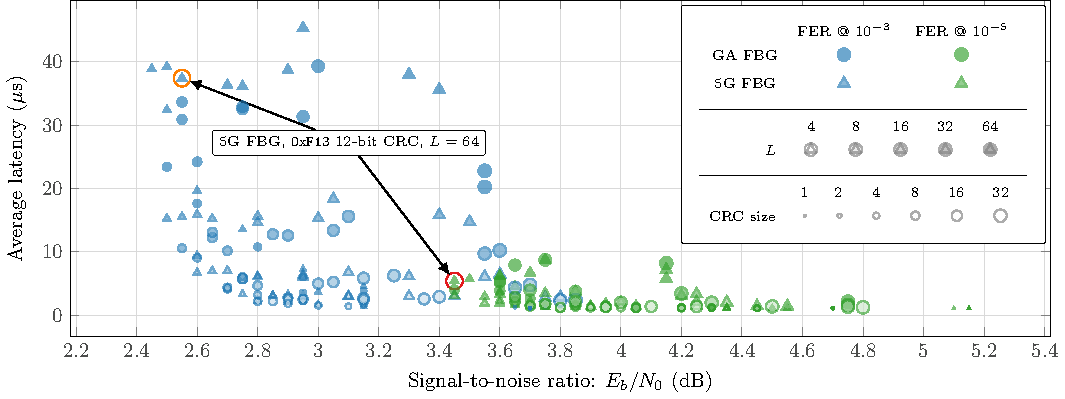
\includegraphics[width=0.85\linewidth]{fig/pareto_k128_r12.pdf}
\caption{Space exploration of the ASCL decoder performance for $K=128$ and $R = 1/2$. Measured latencies from the AFF3CT generic ASCL decoder running on one core of an Intel Xeon Gold 6140 CPU. The selected code is highlighted in \textcolor{Paired_7}{orange} for FER @ $10^{-3}$ and in \textcolor{Paired_5}{red} for FER @ $10^{-5}$.}
  \label{fig:spider_algs}
\end{figure*}

\begin{table*}[h]
\centering
\caption{Proposed codes for the contest with the corresponding achieved performance (fully unrolled ASCL decoders).}
\label{tab:stats}
\resizebox{0.9\columnwidth}{!}{
{\footnotesize
\begin{tabular}{c r r l c c r r r r r}
& & & & & & \multicolumn{5}{c}{Decoder} \\ \cmidrule(lr){7-11}
& & \multicolumn{3}{c}{Code specifications} & \multicolumn{1}{c}{Encoder} & & \multicolumn{2}{c}{FER @ $10^{-3}$} & \multicolumn{2}{c}{FER @ $10^{-5}$} \\ \cmidrule(lr){3-5} \cmidrule(lr){6-6} \cmidrule(lr){8-9} \cmidrule(lr){10-11}
Rate & $K$ & CRC size & CRC poly. & Fb. gen. & $\mathcal{L}_\text{worst}$ ($\mu$s) & $L$ & $E_b/N_0$ & $\mathcal{L}_\text{avg}$ ($\mu$s) & $E_b/N_0$ & $\mathcal{L}_\text{avg}$ ($\mu$s) \\
\midrule
\multirow{4}{*}{$1/4$} &  64 & 11 & \texttt{0x385 } & 5G & 0.20 & 64 &  2.15 dB &  2.53 &  3.35 dB & 0.55 \\
                       & 128 & 12 & \texttt{0xF13 } & 5G & 0.28 & 64 &  1.60 dB &  6.44 &  2.60 dB & 1.07 \\
                       & 256 & 12 & \texttt{0xF13 } & 5G & 0.60 & 64 &  1.25 dB & 10.58 &  2.25 dB & 1.66 \\
                       & 512 & 12 & \texttt{0xF13 } & GA & 1.01 & 32 &  1.10 dB & 14.92 &  1.85 dB & 3.53 \\
\addlinespace
\multirow{4}{*}{$1/2$} &  64 &  7 & \texttt{0x65  } & 5G & 0.14 & 32 &  3.15 dB &  0.70 &  4.60 dB & 0.33 \\
                       & 128 & 12 & \texttt{0xF13 } & 5G & 0.21 & 64 &  2.55 dB &  3.31 &  3.45 dB & 0.69 \\
                       & 256 & 12 & \texttt{0xF13 } & 5G & 0.34 & 64 &  2.15 dB &  6.55 &  3.10 dB & 1.18 \\
                       & 512 & 16 & \texttt{0x8005} & 5G & 0.68 & 64 &  1.90 dB & 11.95 &  2.70 dB & 2.12 \\
\addlinespace
\multirow{4}{*}{$4/5$} &  64 &  8 & \texttt{0x9B  } & GA & 0.15 & 32 &  5.05 dB &  0.48 &  6.45 dB & 0.16 \\
                       & 128 & 10 & \texttt{0x3D9 } & 5G & 0.20 & 32 &  4.40 dB &  1.21 &  5.35 dB & 0.41 \\
                       & 256 & 10 & \texttt{0x3D9 } & 5G & 0.34 & 32 &  4.10 dB &  2.20 &  5.00 dB & 0.67 \\
                       & 512 & 12 & \texttt{0xF13 } & 5G & 0.66 & 32 &  3.75 dB &  4.92 &  4.55 dB & 1.36 \\

\bottomrule
\end{tabular}
}}
\end{table*}

\paragraph{Unrolled ASCL Decoder}
\label{unrolled}
The decoder implemented in this work follows the ASCL decoding principle. This approach aims to reduce the average latency of Polar decoders without compromising error-correction performance. Decoding begins with a fast SC decoder. If the decoded codeword passes the CRC check, it is accepted immediately. Otherwise, the decoder falls back to more powerful SCL decoders with increasing list sizes $L$. This adaptive strategy significantly lowers the average decoding time in high-SNR regimes, where SC decoding is often sufficient, while preserving the robustness of SCL decoding in more challenging conditions. The ASCL mechanism is well suited for short blocklength codes, where latency is critical.

To achieve low latency, we adopt a fully unrolled decoder generation strategy. For each Polar code configuration used in the contest, a dedicated and specialized C++ source file is generated. This eliminates control-flow overhead such as loops and recursive function calls, making the approach particularly effective for short blocklengths where latency is critical.
We provide an open-source decoder generator tool\footnote{Polar decoder generator: https://github.com/aff3ct/polar\_decoder\_gen}, which supports SC, SCL, and ASCL decoding modes. The tool produces optimized C++ code tailored to each frozen set, enabling reproducibility and integration into larger systems.
%TODO citations mcgill & nous

% Pas la place
% - code spécialisé en fonction de la profondeur dans l'arbre -> Polar API
% - code vectorisé en AVX2 quand le nombre d'élément à traiter est supérieur ou égal à 8
% - code vectorisé en SSE quand le nombre d'éléments est exactement égal à 4

% - petit exemple de code généré ?
% - petit schéma du SC pour visualiser la quantité de données en fonction de la profondeur dans le graphe ?

\paragraph{Search space and exploration}
\label{search}

To identify optimal trade-offs for the ISTC 2025 contest, we explored various code and decoder configurations, including different code constructions (GA, 5G)~\cite{Trifonov2012,ETSI2018}, CRC lengths and polynomials -- including some polynomials that do not correspond to standard CRCs -- and list sizes $L$. This search helped uncover ``sweet spots'' balancing latency and error-correction performance. An example of the results obtained for \(K = 128\) and \(N = 256\) is shown in Figure~\ref{fig:spider_algs}.

\paragraph{Performance results}

The testbed was a Minisforum AtomMan X7 Ti PC (Intel Ultra 9 185H, 16 x86-64 cores with 6 p-cores @ 5.1 GHz (one core used), 8 e-cores @ 3.8 GHz (unused), and 2 LPe-cores (unused), 32 GB DDR5 @ 5600 MT/s) running Linux (Ubuntu 25.04 kernel 6.14, g++ 14.2.0) has been used.
Table~\ref{tab:stats} summarizes the proposed Polar code configurations submitted for the contest, along with their measured performance metrics. The table provides details on the code rate, information block length \(K\), CRC size and polynomial, code construction method, worst-case encoder latency, list size \(L\), and decoder performance in terms of Frame Error Rate (FER) at \(10^{-3}\) and \(10^{-5}\) thresholds, together with corresponding average decoding latencies.

\paragraph{1st place and future directions}
The results obtained in the ISTC 2025 contest were very promising, with our submission achieving 1st place in the software implementation category. This success highlights the effectiveness of our approach and the optimizations implemented in the AFF3CT software suite.
The next section is about AFF3CT, its features, and its impact on the field of digital communications. In the end I will also develop our plan to participate in the organization for the next edition of the ISTC contest.

\subsection{The AFF3CT Software Suite}
During my PhD years, followed by a year as an ATER at the University of Bordeaux in the IMS laboratory, a dynamic emerged around the development of a complete software simulation chain, initiated in particular by Adrien Cassagne, then a PhD student in the team. This momentum led to the creation of a software suite named AFF3CT\footnote{https://aff3ct.github.io}\cite{...}. This long-term project (soon to celebrate its 10th anniversary!) has had a strong impact both nationally and internationally, resulting in numerous publications ranging from contributions to software decoders, to the definition of a dedicated programming language for software design, and its use in a variety of application contexts.

For my part, in this document I will focus on the projects in which I was most involved, namely the creation of the chain itself, followed by the implementation of a software radio chain based on the DVB-S2 standard.

\subsubsection{AFF3CT: A Software Suite for Digital Communications}

AFF3CT is an open source software suite designed for the simulation and implementation of communication systems. At the time of its creation, it focused on Monte Carlo simulations of the whole communication chain: some data is generated, encoded, modulated, noised, decoded, and the performance is then estimated by measuring the Bit Error Rate (BER) and the Frame Error Rate (FER). This process led to 3 problems that are addressed by the tool:

\begin{enumerate}
  \item \textbf{Simulation time:} In order to accurately estimate the FER/BER, at least 100 erroneous frames must be simulated. For example, measuring a FER of $10^{-7}$ requires simulating the transmission of approximately $100 \times 10^{7} = 10^{9}$ frames. Assuming a frame length of 1000 bits, the simulator must emulate the transmission of $10^{12}$ bits. Considering that decoding algorithms may be computationally demanding, several weeks or even months of simulation may be required to obtain accurate FER/BER estimates for a given coding scheme.

  \item \textbf{Algorithmic heterogeneity:} A wide variety of channel codes have been developed over time. For each type of code, several decoding algorithms may be available. While describing a single coding scheme is relatively straightforward, providing a unified software framework that supports multiple coding schemes and their associated algorithms is much more challenging. This difficulty stems from the heterogeneity of the data structures required to represent codes and decoders: turbo codes rely on trellises, LDPC codes are naturally expressed on factor graphs, and polar codes are efficiently decoded using binary trees.

  \item \textbf{Reproducibility:} Reproducing published results is often a tedious task. This is partly due to the large number of empirical parameters required to specify a communication system, not all of which are systematically reported in publications. Moreover, simulator source codes are rarely made publicly available. As a consequence, significant time is frequently spent ``reinventing the wheel'' merely to enable comparison with state-of-the-art results.
\end{enumerate}



The long simulation times make it desirable to have \textbf{high throughput
implementations}. The algorithmic heterogeneity requires \textbf{flexible,
modular software}. The reproducibility issue pushes towards a \textbf{portable}
and \textbf{open-source software}. These are the purposes of \AFFECT.

\subsubsection{Related Works}

\begin{table}[htp]
\centering
\caption{\texttt{C}/\Cxx open source channel coding simulators/libraries.}
\label{tab:libraries}
{\small\resizebox{\linewidth}{!}{
\begin{tabular}{c | r | r | r | r | c | C{\simcolwidth}  C{\simcolwidth}  C{\simcolwidth}  C{\simcolwidth}  C{\simcolwidth}  C{\simcolwidth}  C{\simcolwidth}  C{\simcolwidth}  C{\simcolwidth}  C{\simcolwidth} }
  \multirow{4}{*}{\textbf{Name}}                                                      &                  & \multirow{4}{*}{\textbf{Lines}} & \multicolumn{2}{c |}{\multirow{2}{*}{\textbf{Commit}}}           & \multirow{4}{*}{\textbf{License}} & \multirow{4}{*}{\rotatebox[origin=c]{70}{Polar}} & \multirow{4}{*}{\rotatebox[origin=c]{70}{LDPC}} & \multirow{4}{*}{\rotatebox[origin=c]{70}{Turbo}} & \multirow{4}{*}{\rotatebox[origin=c]{70}{Turbo P.}} & \multirow{4}{*}{\rotatebox[origin=c]{70}{BCH}} & \multirow{4}{*}{\rotatebox[origin=c]{70}{RS}} & \multirow{4}{*}{\rotatebox[origin=c]{70}{Conv.}} & \multirow{4}{*}{\rotatebox[origin=c]{70}{RA}} & \multirow{4}{*}{\rotatebox[origin=c]{70}{Rep.}} & \multirow{4}{*}{\rotatebox[origin=c]{70}{Erasure}} \\
                                                                                      & \textbf{Contri-} &                                 & \multicolumn{2}{c |}{}                                           &                                   &        &        &        &        &        &        &        &        &        &         \\ \cline{4-5}
                                                                                      & \textbf{butors}  &                                 & \multirow{2}{*}{\textbf{First}} & \multirow{2}{*}{\textbf{Last}} &                                   &        &        &        &        &        &        &        &        &        &         \\
                                                                                      &                  &                                 &                                 &                                &                                   &        &        &        &        &        &        &        &        &        &         \\ \hline
                                                                                                                                                                                                                                                  % Polar    LDPC     Turbo    TPC      BCH      RS       Conv.    RA       Rep.     Erasure
  \href{https://github.com/aff3ct/aff3ct                   }{\texttt{AFF3CT}}         &               11 &                             76k & 2016                            & 2019                           & MIT                               & \cmark & \cmark & \cmark & \cmark & \cmark & \cmark & \cmark & \cmark & \cmark & \xmark  \\
  \href{http://www.eccpage.com/                            }{\texttt{eccpage}}        &               20 &                               - & 1989                            & 2006                           & -                                 & \xmark & \cmark & \cmark & \xmark & \cmark & \cmark & \cmark & \xmark & \xmark & \cmark  \\
  \href{https://github.com/pjkundert/ezpwd-reed-solomon    }{\texttt{EZPWD}}          &                2 &                              6k & 2014                            & 2018                           & GPLv3                             & \xmark & \xmark & \xmark & \xmark & \xmark & \cmark & \xmark & \xmark & \xmark & \xmark  \\
  \href{https://github.com/Bulat-Ziganshin/FastECC         }{\texttt{FastECC}}        &                2 &                              1k & 2015                            & 2018                           & Apache 2.0                        & \xmark & \xmark & \xmark & \xmark & \xmark & \cmark & \xmark & \xmark & \xmark & \xmark  \\
  \href{https://github.com/catid/fecal                     }{\texttt{FEC-AL}}         &                1 &                              3k & 2018                            & 2018                           & BSD 3-Clause                      & \xmark & \xmark & \xmark & \xmark & \xmark & \xmark & \cmark & \xmark & \xmark & \cmark  \\
  \href{https://github.com/randombit/fecpp                 }{\texttt{FECpp}}          &                1 &                              2k & 2009                            & 2018                           & -                                 & \xmark & \xmark & \xmark & \xmark & \xmark & \xmark & \xmark & \xmark & \xmark & \cmark  \\
  \href{https://github.com/gnuradio/gnuradio               }{\texttt{GNURadio}}       &              192 &                            270k & 2006                            & 2019                           & GPLv3                             & \cmark & \cmark & \xmark & \xmark & \xmark & \xmark & \cmark & \xmark & \cmark & \xmark  \\
  \href{http://itpp.sourceforge.net                        }{\texttt{IT++}}           &               20 &                            109k & 2005                            & 2018                           & GPLv3                             & \xmark & \cmark & \cmark & \xmark & \cmark & \cmark & \cmark & \xmark & \xmark & \xmark  \\
  \href{https://github.com/blegal/Fast_LDPC_decoder_for_x86}{\texttt{LeGal}}          &                1 &                             83k & 2015                            & 2019                           & -                                 & \xmark & \cmark & \xmark & \xmark & \xmark & \xmark & \xmark & \xmark & \xmark & \xmark  \\
  \href{https://github.com/catid/leopard                   }{\texttt{Leopard}}        &                4 &                              5k & 2017                            & 2018                           & BSD 3-Clause                      & \xmark & \xmark & \xmark & \xmark & \xmark & \cmark & \xmark & \xmark & \xmark & \xmark  \\
  \href{https://github.com/quiet/libcorrect                }{\texttt{libcorrect}}     &                6 &                              5k & 2016                            & 2018                           & BSD 3-Clause                      & \xmark & \xmark & \xmark & \xmark & \xmark & \cmark & \cmark & \xmark & \xmark & \xmark  \\
  \href{https://gitlab.eurecom.fr/oai/openairinterface5g   }{\texttt{OpenAir}}        &              148 &                            740k & 2013                            & 2019                           & OAI Public                        & \xmark & \xmark & \cmark & \xmark & \xmark & \xmark & \xmark & \xmark & \xmark & \xmark  \\
  \href{http://openfec.org/                                }{\texttt{OpenFEC}}        &                8 &                             55k & 2009                            & 2014                           & CeCCIL-C                          & \xmark & \cmark & \xmark & \xmark & \xmark & \cmark & \xmark & \xmark & \xmark & \xmark  \\
  \href{https://github.com/ArashPartow/schifra             }{\texttt{Schifra}}        &                1 &                              7k & 2010                            & 2018                           & GPLv3                             & \xmark & \xmark & \xmark & \xmark & \xmark & \cmark & \xmark & \xmark & \xmark & \xmark  \\
  \href{https://github.com/catid/siamese                   }{\texttt{Siamese}}        &                1 &                             11k & 2018                            & 2018                           & BSD 3-Clause                      & \xmark & \xmark & \xmark & \xmark & \xmark & \xmark & \cmark & \xmark & \xmark & \cmark  \\
  \href{https://github.com/tavildar/Polar                  }{\texttt{Tavildar-Polar}} &                1 &                              2k & 2016                            & 2017                           & -                                 & \cmark & \xmark & \xmark & \xmark & \xmark & \xmark & \xmark & \xmark & \xmark & \xmark  \\
  \href{https://github.com/tavildar/LDPC                   }{\texttt{Tavildar-LDPC}}  &                1 &                              1k & 2016                            & 2016                           & -                                 & \xmark & \cmark & \xmark & \xmark & \xmark & \xmark & \xmark & \xmark & \xmark & \xmark  \\
  \href{http://www.the-art-of-ecc.com                      }{\texttt{the-art-of-ecc}} &                1 &                               - & 2006                            & 2009                           & Copyright                         & \xmark & \cmark & \cmark & \cmark & \cmark & \cmark & \cmark & \xmark & \xmark & \xmark  \\
  \href{https://github.com/ttsou/turbofec                  }{\texttt{TurboFEC}}       &                2 &                              4k & 2015                            & 2018                           & GPLv3                             & \xmark & \xmark & \cmark & \xmark & \xmark & \xmark & \xmark & \xmark & \xmark & \xmark  \\
  \end{tabular}
}}
\end{table}

In the digital communications community, many scientists implement their own
simulation chain to validate their works. Table~\ref{tab:libraries} presents, to
the best of our knowledge, a list of currently available \verb|C|/\Cxx open
source channel coding simulators/libraries. We choose to compare with projects
compiled as binaries, since they aim at high throughput and low latency,
as \AFFECT. Many open source projects in Python or in MATLAB exist as well, but
these tools are usually slower than compiled binaries, and rather aim at
prototyping.

Table~\ref{tab:libraries} shows that, generally, the \verb|C|/\Cxx FEC libraries
target a single family or a small subset of channel codes. As a consequence, a
large effort is spent to re-develop similar features, since all those libraries
and tools share many characteristics (except the channel code itself). \AFFECT
attempts to lower this redundancy by releasing a full simulator/library that
consistently supports a wide range of channel codes to the community. \AFFECT
also tries to homogenize usage (command line, \Cxx interfaces, etc.) for all
code families. Table~\ref{tab:libraries} does not aim at comparing channel code
implementation performances. Instead, on the \AFFECT website, an overview of
software channel decoders state-of-the-art is provided for turbo, LDPC and polar
codes\footnote{FEC Software Decoders Hall of Fame: \url{http://aff3ct.github.io/hof_turbo.html}}.

\subsubsection{Software description}
\label{}

\AFFECT is a Forward Error Correction (FEC) toolbox. The most important tools
it includes are the \textit{simulator} and the \textit{library}. Additionally,
the toolbox comes with a bank of \textit{simulated references}, a
\textit{GUI software} to browse those references, and a set of predefined
\textit{configuration files} for common communication standards.

\paragraph{Simulator}

\begin{figure}[htp]
    \centering
    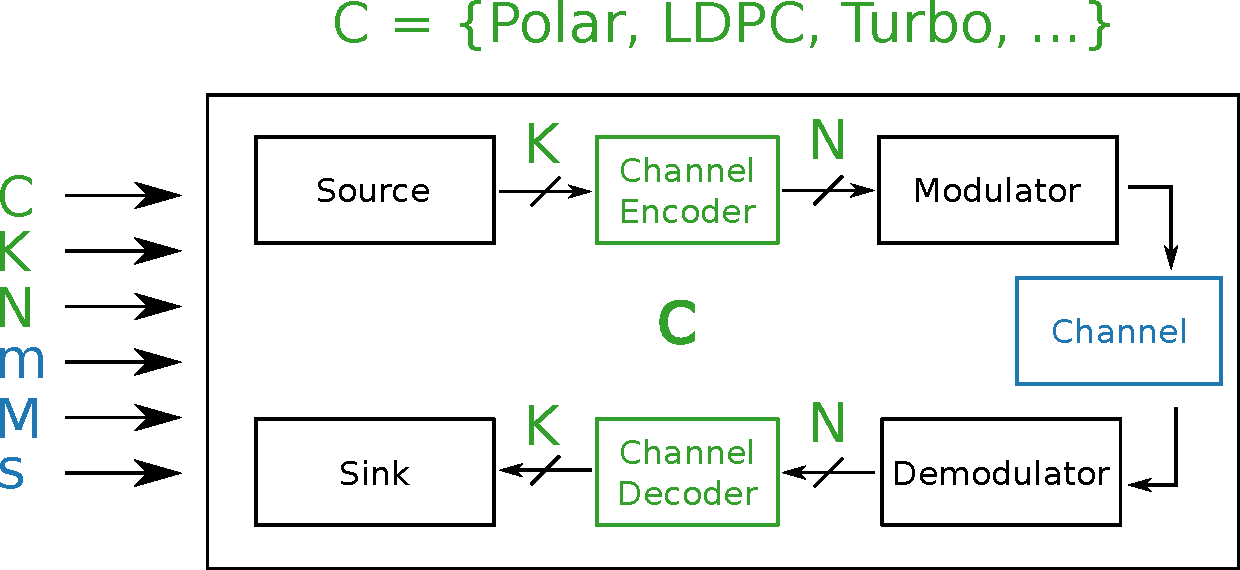
\includegraphics[scale=0.400]{fig/codeoptions.pdf}
    \caption{Main simulation parameters.}
    \label{fig:code_options}
\end{figure}

\begin{figure}[htp]
    \centering
    \begin{subfigure}[t]{0.32\textwidth}
        \centering
        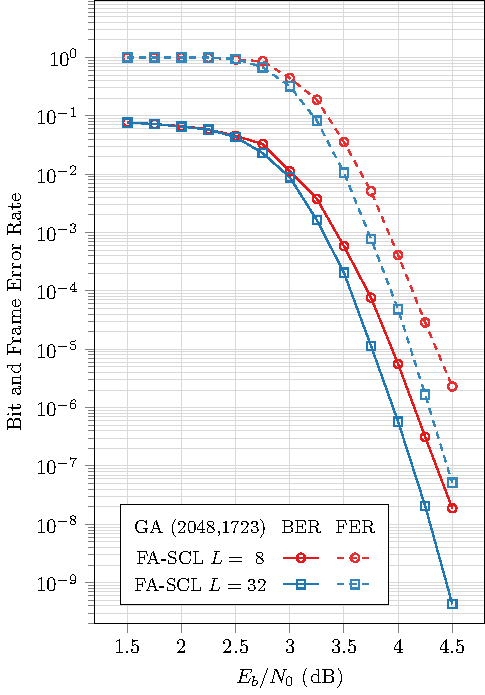
\includegraphics[width=1.0\textwidth]{fig/bfer_polar}
        \caption{Polar codes.}
        \label{fig:code_polar}
    \end{subfigure}
    %
    \begin{subfigure}[t]{0.32\textwidth}
        \centering
        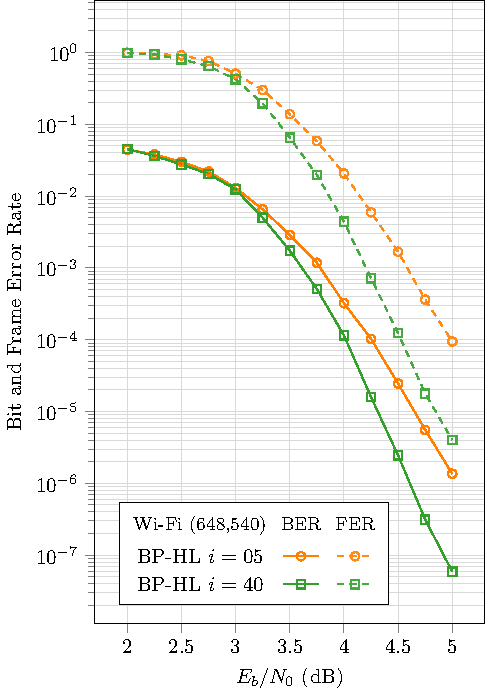
\includegraphics[width=1.0\textwidth]{fig/bfer_ldpc}
        \caption{LDPC codes.}
        \label{fig:code_ldpc}
    \end{subfigure}
    %
    \begin{subfigure}[t]{0.32\textwidth}
        \centering
        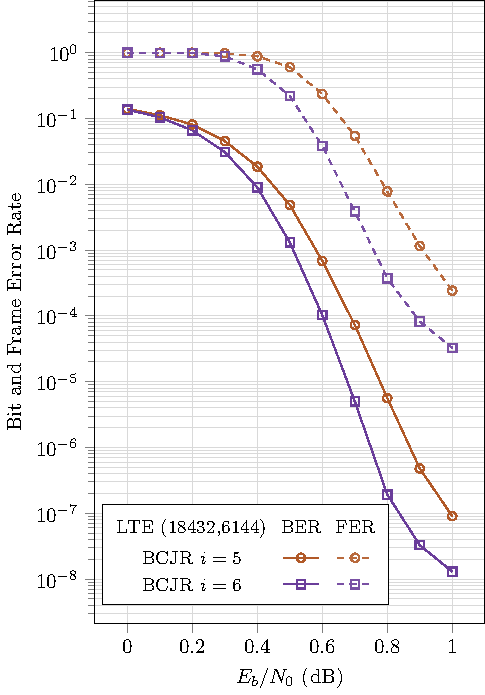
\includegraphics[width=1.0\textwidth]{fig/bfer_turbo}
        \caption{Turbo codes.}
        \label{fig:code_turbo}
    \end{subfigure}
    %
    \begin{subfigure}[b]{0.32\textwidth}
        \centering
        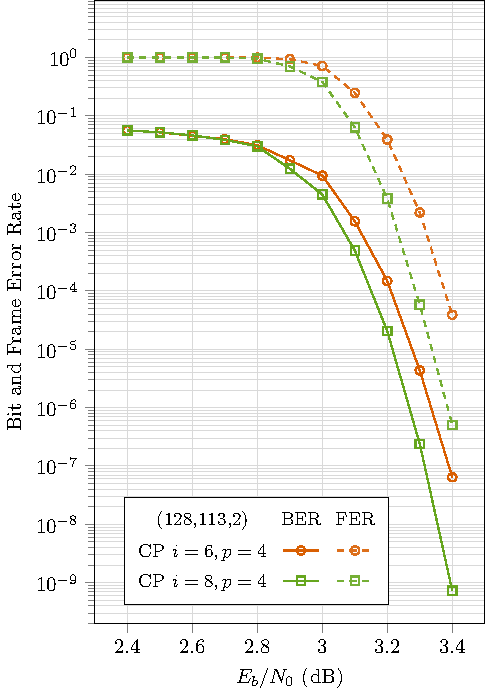
\includegraphics[width=1.0\textwidth]{fig/bfer_tpc}
        \caption{Turbo product codes.}
        \label{fig:code_tpc}
    \end{subfigure}
     %
    \begin{subfigure}[b]{0.32\textwidth}
        \centering
        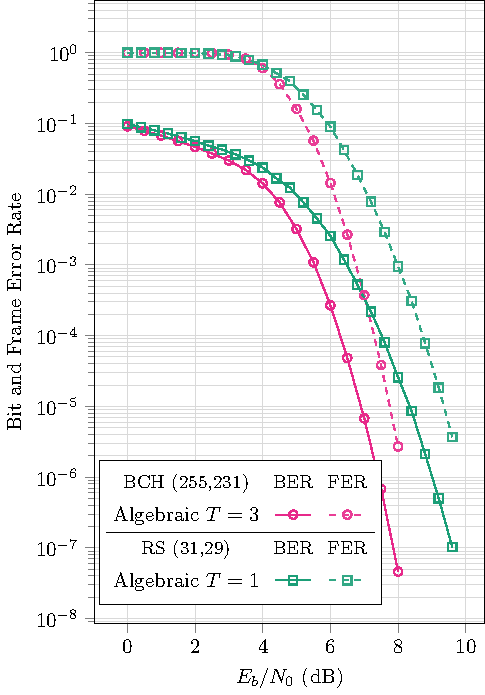
\includegraphics[width=1.0\textwidth]{fig/bfer_bch_rs}
        \caption{BCH \& RS codes.}
        \label{fig:code_bch_rs}
    \end{subfigure}
     %
    \begin{subfigure}[b]{0.32\textwidth}
        \centering
        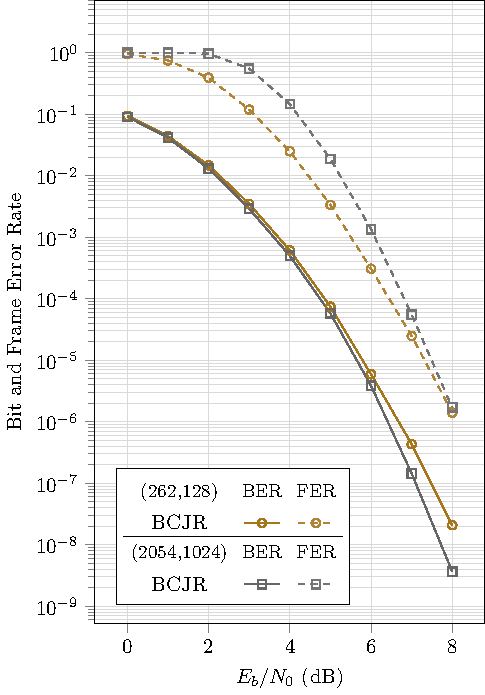
\includegraphics[width=1.0\textwidth]{fig/bfer_rsc}
        \caption{Convolutional codes.}
        \label{fig:code_rsc}
    \end{subfigure}
    \caption{\AFFECT simulation of various code families.}
    \label{fig:code_all}
\end{figure}

As a standalone simulator, \AFFECT proposes to simulate various communication
chains with a broad range of codes. The simulator is a command line program;
Figure~\ref{fig:code_options} depicts its main arguments: \verb|-m| and
\verb|-M| set the minimum and the maximum Signal Noise Ratio (SNR, $E_b/N_0$) to
simulate, \verb|-s| specifies the iteration step inbetween. Parameter \verb|-C|
selects the channel code type, \verb|-K| sets the length in bits of the initial
information message and \verb|-N| sets the codeword size, which is the encoder
output size\footnote{The \AFFECT simulator comes with many more options, omitted
here for concision.}. The command line interface is designed to be easily used
from scripts. Figure~\ref{fig:code_all} shows simulations ran with \AFFECT on
various code types (BPSK modulation and AWGN channel).

\subsubsection{Library}

As a FEC library, \AFFECT can be used programmatically, for instance in
\emph{Software Defined Radio} (SDR) contexts or in simulations. \AFFECT blocks
can be used in external projects without restriction. Compute intensive blocks
are optimized and vectorized to run fast on a single core. The library is
thread-safe; however, it is not multi-threaded by itself, in contrast to the
simulator. Instead, it is the responsibility of the user to manage
multi-threading.

\subsubsection{Software Architecture}
\label{sec:soft_archi}

\AFFECT is developed in \Cxx in an object-oriented programming style. It
provides the fundamental blocks involved in building communication chains
(sources, modems, codecs, channels, ...). Those blocks are organized as
\textit{modules} and \textit{tasks}.

\textbf{Module:} A set of related tasks sharing some characteristics. For
instance, the \textit{modem} module contains the \textit{modulate} and
\textit{demodulate} tasks.

\textbf{Task:} An elementary processing performed on some data. For instance,
\textit{decode} or \textit{modulate} are tasks. The tasks are characterized by
their \textit{sockets}. A socket of a task defines an entry point through which
the task will consume and/or produce data. There are three kinds of sockets:
\textit{input}, \textit{output} and \textit{input/output}, following a
philosophy close to \emph{ports} in component-based development approaches.

\begin{figure}[htp]
  \centering
  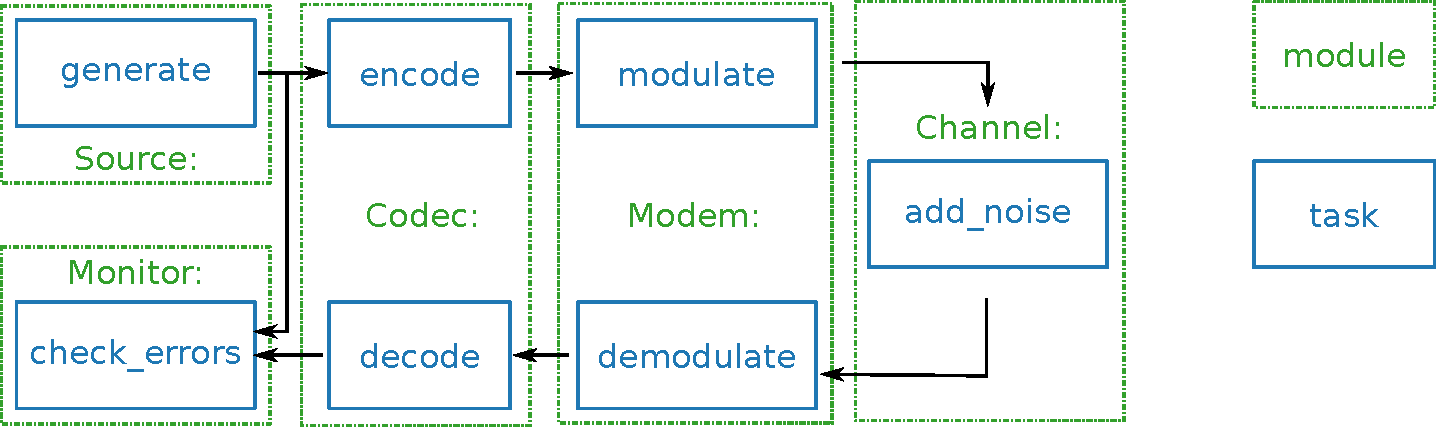
\includegraphics[scale=0.400]{fig/tasks_modules.pdf}
  \caption{Modules and tasks.}
  \label{fig:modules_tasks}
\end{figure}

As a rule, a task is always a \emph{verb} and a module is always a \emph{noun}.
Modules are implemented as C++ classes, and tasks as class methods. \AFFECT
defines several abstract modules, for sources, codecs, modems, channels, etc. It
readily provides many implementations of those abstract classes; it is also
straightforward to add new ones. Figure~\ref{fig:modules_tasks} presents common
modules and tasks typically found in a basic communication chain. It shows that
the number of tasks per module can vary depending on the module type.

\subsubsection{Software Functionalities}
\label{}

The \AFFECT software functionalities can be decomposed in three main parts: the
\textit{codecs}, the \textit{modems} and the \textit{channels}. The codecs are
the main part of the toolbox. There is a broad range of supported codes listed
in Table~\ref{tab:codecs}.

\begin{table}[htp]
\centering
\caption{List of supported channel codes (codecs).}
\label{tab:codecs}
{\footnotesize%\resizebox{\linewidth}{!}{
\begin{tabular}{| c | c | c |}
  \hline
  \multirow{2}{*}{\textbf{Channel Code}}   & \multirow{2}{*}{\textbf{Standards}} & \multirow{2}{*}{\textbf{Decoders}}     \\
                                           &                                     &                                        \\
  \hline
  \multirow{5}{*}{\textbf{LDPC}}           & 5G (data), WiFi,                    & Scheduling: Flooding and H./V. Layered \\
                                           & WiMAX, WRAN,                        & Sum-Product Algorithm (SPA)            \\
                                           & 10 Gigabit Eth.,                    & Min-Sum (NMS, OMS)                     \\
                                           & DVB-S2, CCSDS                       & Approximate Min-Star (AMS)             \\
                                           & etc.                                & Bit Flipping: GallagerA/B/E, PPBF, WBF \\
  \hline
  \multirow{4}{*}{\textbf{Polar}}          &                                     & Successive Cancellation (SC)           \\
                                           & 5G                                  & Successive Cancellation List (SCL)     \\
                                           & (control channel)                   & CRC Aided SCL (CA-SCL, Adaptive SCL)   \\
                                           &                                     & Soft Cancellation (SCAN)               \\
  \hline
  \multirow{1}{*}{\textbf{Turbo Parallel}} & LTE (3G, 4G),                       & Turbo BCJR                             \\
  (single and double                       & DVB-RCS,                            & Turbo BCJR + Early Termination (CRC)   \\
  binary)                                  & CCSDS, etc.                         & Post proc.: Flip aNd Check (FNC)       \\
  \hline
  \multirow{2}{*}{\textbf{Turbo Product}}  & \multirow{2}{*}{WiMAX (opt.)}       & \multirow{2}{*}{Turbo Chase-Pyndiah}   \\
                                           &                                     &                                        \\
  \hline
  \multirow{3}{*}{\textbf{BCH}}            & CD, DVD,                            &                                        \\
                                           & SSD, DVB-S2,                        & Berlekamp-Massey + Chien search        \\
                                           & Bitcoin, etc.                       &                                        \\
  \hline
  \multirow{3}{*}{\textbf{Reed-Solomon}}   & CD, DVD,                            &                                        \\
                                           & SSD, DVB-T,                         & Berlekamp-Massey + Chien search        \\
                                           & ADSL, etc.                          &                                        \\
  \hline
  \multirow{1}{*}{\textbf{Convolutional}}  &                                     & BCJR - Maximum A Posteriori (MAP)      \\
  (single and double                       & NASA                                & BCJR - Linear Approximation            \\
  binary)                                  &                                     & BCJR - Max Approximation               \\
  \hline
  \end{tabular}
}%}
\end{table}

The codecs naturally encompass the encoders and decoders, but they can also
include puncturing patterns to shorten frames length according to some
communication standards. Most of the codec algorithms come from the literature,
while the others have been designed under
\AFFECT~\cite{Tonnellier2016a,Tonnellier2016b,Tonnellier2016,leonardon:hal-01987848}.
In channel coding, the decoder is the most time-consuming process, compared to
the puncturing and the encoding processes. This is why a specific effort is put
on ensuring the high computing performance of the decoders. Most of the decoding
algorithms have thus been optimized to satisfy high throughput and low latency
constraints~\cite{LeGal2015a,Cassagne2015c,Cassagne2016a,Cassagne2016b}. Those
optimizations generally involve a vectorized implementation, a tailored data
quantization and the use of fixed-point arithmetic.

In typical communication chains, it is necessary to adapt the digital signal
to the physical support. This operation is performed by the modulator and
conversely by the demodulator. \AFFECT comes with a rich set of modems to this
purpose. Table~\ref{tab:modems} lists all the supported modems.

\begin{table}[htp]
\centering
\caption{List of supported modulations/demodulations (modems).}
\label{tab:modems}
{\footnotesize%\resizebox{\linewidth}{!}{
\begin{tabular}{| c | c | c |}
  \hline
  \multirow{2}{*}{\textbf{Modem}}        & \multirow{2}{*}{\textbf{Standard}} & \multirow{2}{*}{\textbf{Characteristics}} \\
                                         &                                    &                                           \\
  \hline
  \multirow{3}{*}{\textbf{N-PSK}}        & IEEE 802.16 (WiMAX)                &                                           \\
                                         & UMTS (2G, 2G+)                     & Phase-Shift Keying                        \\
                                         & EDGE (8-PSK), ...                  &                                           \\
  \hline
  \multirow{3}{*}{\textbf{N-QAM}}        & IEEE 802.16 (WiMAX)                &                                           \\
                                         & UMTS (2G, 2G+)                     & Quadrature Amplitude Modulation           \\
                                         & 3G, 4G, 5G, ...                    &                                           \\
  \hline
  \multirow{3}{*}{\textbf{N-PAM}}        & IEEE 802.16 (WiMAX)                &                                           \\
                                         & UMTS (2G, 2G+)                     & Pulse Amplitude Modulation                \\
                                         & 3G, 4G, 5G, ...                    &                                           \\
  \hline
  \multirow{2}{*}{\textbf{CPM}}          & GMSK, Bluetooth                    & Continuous Phase Modulation               \\
                                         & IEEE 802.11 FHSS                   & Coded (convolutional-based) modulation    \\
  \hline
  \multirow{2}{*}{\textbf{OOK}}          & IrDA (Infrared)                    & On-Off Keying                             \\
                                         & ISM bands                          & Used in optical communication systems     \\
  \hline
  \multirow{2}{*}{\textbf{SCMA}}         & \multirow{2}{*}{Considered for 5G} & Sparse Code Multiple Access               \\
                                         &                                    & Multi-user modulation                     \\
  \hline
  \multirow{2}{*}{\textbf{User defined}} & \multirow{2}{*}{-}                 & Constellation and order can be            \\
                                         &                                    & defined from an external file             \\
  \hline
  \end{tabular}
}%}
\end{table}

\AFFECT supports several coded modulation/demodulation schemes like the
Continuous Phase Modulation (CPM)~\cite{Aulin1981a,Aulin1981b} and the Sparse
Code Multiple Access (SCMA) modulation~\cite{Nikopour2013,Ghaffari2017,Ghaffari2019}
(many codebooks are supported~\cite{Altera,Wu2015,Cheng2015,Zhang2016,Klimentyev2016,SongWC2016,Klimentyev2017}).
It allows to easily combine and evaluate the channel codes with several types
of modulations. In the case of the CPM, analogical wave shapes are also
simulated. The other modulation schemes are at the digital level.

For simulation purposes, it is crucial to emulate the behavior of the physical
layer. This is the role of the channel. There are many possible configurations
depending on the physics phenomena to simulate. Table~\ref{tab:channels}
reports all the supported channels.

\begin{table}[htp]
\centering
\caption{List of supported channels.}
\label{tab:channels}
{\footnotesize%\resizebox{\linewidth}{!}{
\begin{tabular}{| c | c | c | c |}
  \hline
  \multirow{2}{*}{\textbf{Channel}}      & \multirow{2}{*}{\textbf{Multi-user}} & \multirow{2}{*}{\textbf{Characteristics}}      \\
                                         &                                      &                                                \\
  \hline
  \multirow{2}{*}{\textbf{AWGN}}         & \multirow{2}{*}{Yes}                 & \multirow{2}{*}{Additive White Gaussian Noise} \\
                                         &                                      &                                                \\
  \hline
  \multirow{2}{*}{\textbf{BEC}}          & \multirow{2}{*}{No}                  & \multirow{2}{*}{Binary Erasure Channel}        \\
                                         &                                      &                                                \\
  \hline
  \multirow{2}{*}{\textbf{BSC}}          & \multirow{2}{*}{No}                  & \multirow{2}{*}{Binary Symmetric Channel}      \\
                                         &                                      &                                                \\
  \hline
  \multirow{2}{*}{\textbf{Rayleigh}}     & \multirow{2}{*}{Yes}                 & \multirow{2}{*}{Flat Rayleigh fading channel}  \\
                                         &                                      &                                                \\
  \hline
  \multirow{2}{*}{\textbf{User defined}} & \multirow{2}{*}{Not yet}             & User can import noise samples                  \\
                                         &                                      & from an external file                          \\
  \hline
  \end{tabular}
}%}
\end{table}

The channels involve complex floating-point computations. It is frequent to use
exponential and trigonometric operations. Those types of operations cost a large
amount of CPU cycles to be computed. As for the decoders, the channels have been
carefully optimized based on branch instructions reduction and massive
vectorization.

All these features are available from the simulator and in the library. Many
additional functional functionalities available are skipped here for concision.

\subsubsection{Software Continuous Integration}

\AFFECT's development leverages streamlined Continuous Integration (CI) process.
Each new commit to the version control repository triggers a comprehensive
sequence of tests to catch potential regressions. Regression tests are based on
past simulation results, validated from the state-of-the-art.

The CI process enables us to safely and confidently integrate contributed
features and improvements from the community to \AFFECT. It also helps to keep
the code review time by the core development team low-enough to swiftly
integrate such contributions into the master branch.


\subsubsection{A Flexible and Portable Real-time DVB-S2 Transceiver using Multicore and SIMD CPUs}
\begin{figure*}[t]
  \centering
  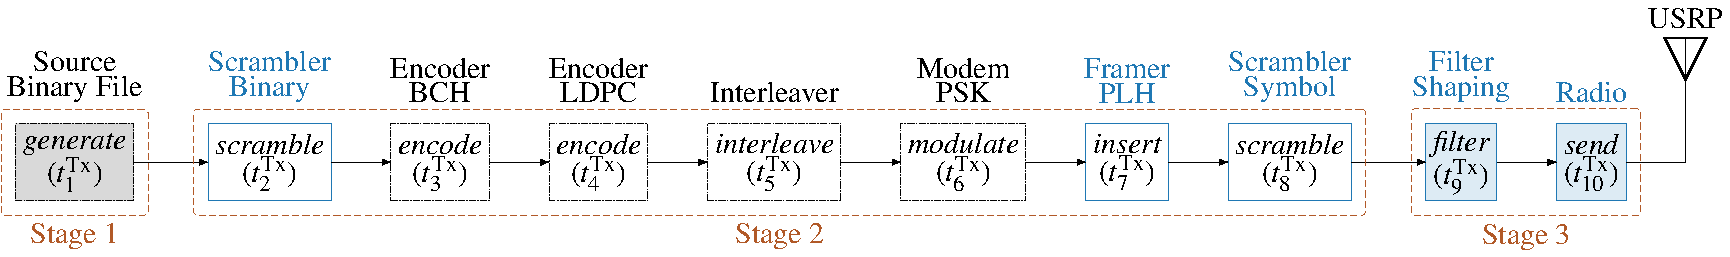
\includegraphics[width=0.90\textwidth]{fig/transmitter}
  \caption
    [DVB-S2 transmitter software implementation.]
    {DVB-S2 transmitter software implementation.}
  \label{fig:sdr_dvbs2_transmitter}
\end{figure*}
\begin{figure*}[t]
  \centering
  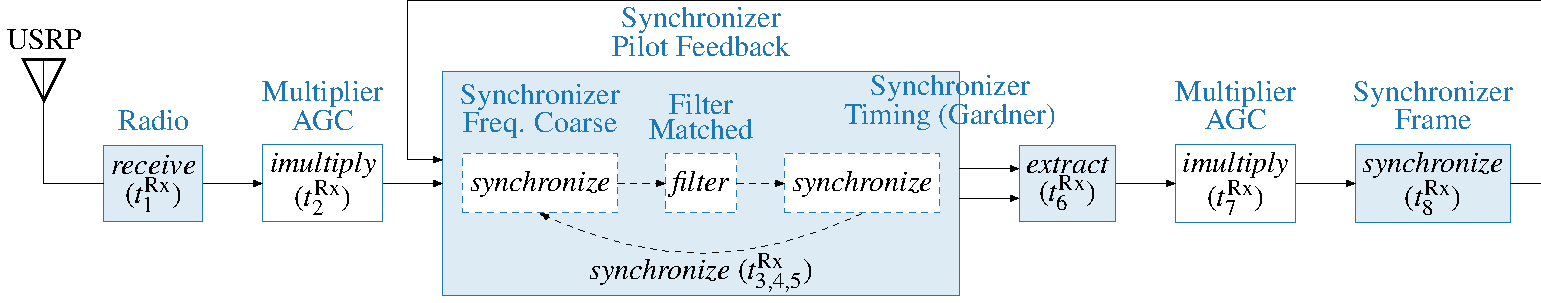
\includegraphics[width=0.72\linewidth]{fig/receiver_learning}
  \caption{DVB-S2 software receiver: waiting phase and acquisition phase 1 \& 2.}
  \label{fig:sdr_dvbs2_receiver_learning}
\end{figure*}

\begin{figure*}[t]
  \centering
  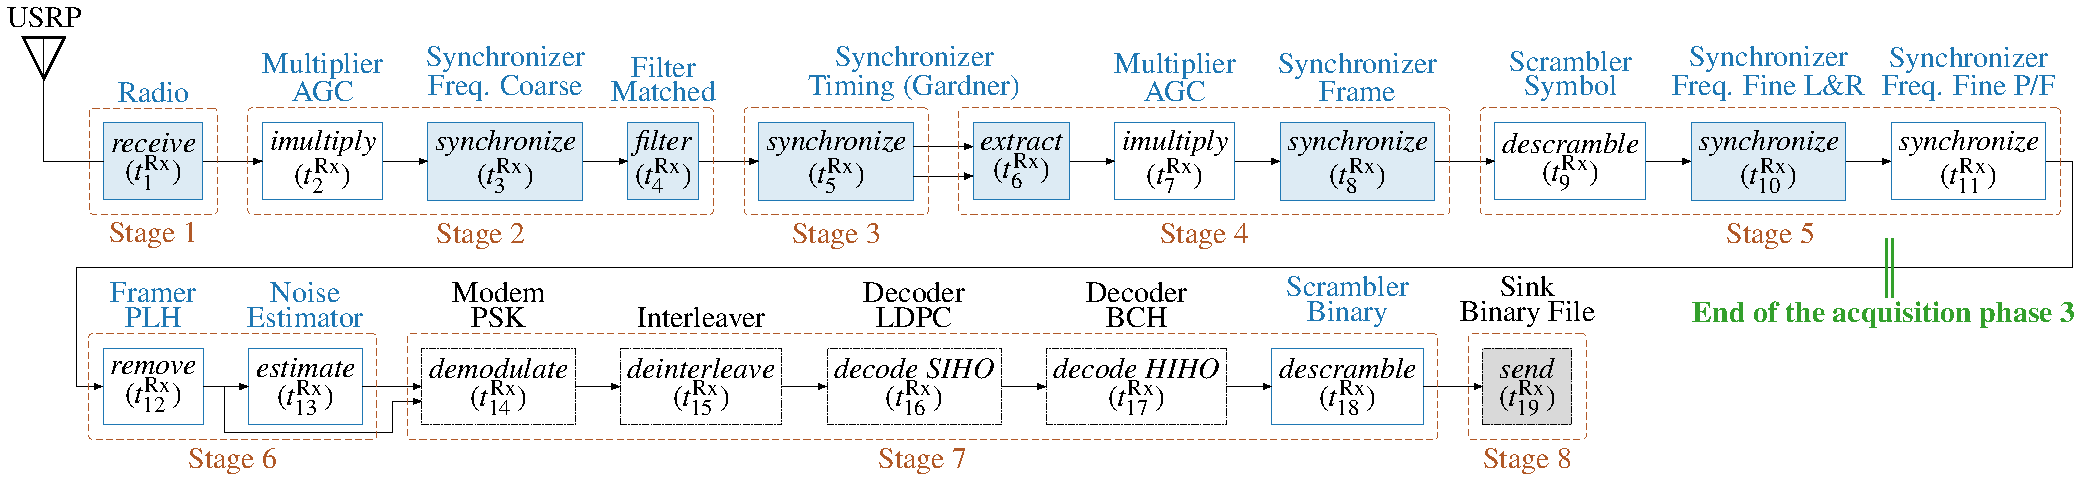
\includegraphics[width=1.0\linewidth]{fig/receiver_transmission}
  \caption{DVB-S2 software receiver: acquisition phase 3 \& transmission phase.}
  \label{fig:sdr_dvbs2_receiver_transmission}
\end{figure*}

During my ATER position at the University of Bordeaux, our research group was
contacted by Airbus Defense and Space to develop a software-defined radio (SDR)
implementation of the DVB-S2 standard. The goal was to create a real-time
demonstrator capable of streaming video over Universal Software Radio Peripheral
(USRP) platforms. This demonstrator serves to showcase the \AFFECT toolbox and
its capabilities in practical SDR applications.

The collaboration led to the development of a complete end-to-end DVB-S2
transceiver, including both the transmission and reception chains. In addition
to implementing the standard coding and modulation schemes, a key contribution
of this work was the integration of robust synchronization functionalities,
which were not available in \AFFECT at the time. This enabled reliable frame,
timing, and frequency recovery under real-world transmission conditions. The
developed system is still used today to demonstrate \AFFECT toolsuite features
and to illustrate high-performance SDR processing on general-purpose multicore
CPUs.

Software implementations of digital communication standards such as DVB-S2 are
particularly relevant in satellite ground stations. They offer flexibility,
hardware mutualization, and maintainability advantages over dedicated hardware
solutions, especially when the production volume is low or when the system must
adapt to evolving standards. However, achieving real-time performance in
software is challenging, as the system must process tens of megabits per second
with minimal latency while compensating for imperfections in the transmission
chain, such as frequency offsets and timing drifts.

In this context, the proposed SDR implementation combines the flexibility of
software with the performance required for real-time operations. It relies on
the parallelism of multicore CPUs and Single Instruction Multiple Data (SIMD)
vectorization to accelerate processing tasks. The demonstrator supports multiple
DVB-S2 MODulation and CODing schemes (MODCODs) and provides precise
synchronization through dedicated software modules.

The remainder of this section presents the overall DVB-S2 transceiver
architecture, detailing the transmission and reception chains as illustrated in
Figs.~\ref{fig:sdr_dvbs2_transmitter},~\ref{fig:sdr_dvbs2_receiver_learning}
and~\ref{fig:sdr_dvbs2_receiver_transmission}. This description emphasizes both
the processing steps inherited from \AFFECT and the newly implemented modules
for synchronization, filtering, and real-time sample handling.

\subsubsection{DVB-S2 Transceiver Overview}


The developed DVB-S2 transceiver is composed of two main parts: the transmitter
and the receiver, both implemented in software and interfaced with USRP
hardware for analog signal transmission and reception. The design follows a
modular approach, where each processing task is clearly separated and can be
optimized or parallelized independently.

\paragraph{Transmitter Architecture}

The transmitter chain, illustrated in Fig.~\ref{fig:sdr_dvbs2_transmitter},
reads the source data and applies the DVB-S2 processing steps, including
encoding, modulation, and optional interleaving. Additional tasks such as
scrambling, pilot insertion, and shaping filtering ensure that the transmitted
signal meets the standard requirements and facilitates synchronization at the
receiver. Some tasks rely directly on existing \AFFECT modules, while others
have been implemented specifically for the SDR context, allowing real-time
transmission through the USRP.

\paragraph{Receiver Architecture}

The receiver chain, depicted in
Figs.~\ref{fig:sdr_dvbs2_receiver_learning}~and~\ref{fig:sdr_dvbs2_receiver_transmission},
follows a phased processing approach. Initially, the receiver waits for an
incoming signal and performs acquisition in several stages to estimate timing,
frequency, and frame alignment. Once synchronization is achieved, the
transmission phase begins, in which the incoming frames are processed in real
time through the full DVB-S2 decoding chain.

Dedicated synchronization tasks ensure resilience to frequency offsets, timing
drifts, and phase variations in the received signal. These tasks, along with
filters and frame extractors, were newly implemented for this SDR demonstrator
and are integrated with the \AFFECT interfaces, providing a modular and
instrumented software architecture.

\paragraph{Key Features}

The SDR implementation highlights several important aspects:

\begin{itemize}
  \item \textbf{Real-time processing:} The receiver pipeline is carefully
        parallelized and optimized to handle the high data rates imposed by the
        USRP modules.
  \item \textbf{Flexible and modular design:} The transceiver architecture
        separates tasks in a way that facilitates adaptation to different
        MODCODs and transmission scenarios.
  \item \textbf{Synchronization:} Custom software modules compensate for
        timing and frequency drifts, enabling robust reception under realistic
        conditions.
  \item \textbf{Integration with \AFFECT:} The design leverages the toolbox for
        core signal processing and decoding tasks, while extending it with SDR
        specific functionality.
\end{itemize}

This high-level architecture demonstrates that a software-only DVB-S2
transceiver can meet real-time constraints using general-purpose CPUs,
multicore parallelism, and SIMD acceleration, while remaining fully modular and
extensible.
\subsubsection{Real-Time Implementation Features}
\label{sec:real_time_summary}

Achieving real-time performance for a software DVB-S2 transceiver requires
careful management of data flow, processing parallelism, and hardware
capabilities. In our SDR demonstrator, the following key strategies were applied:

\paragraph{Reliable Sample Collection and Delivery}

The USRP modules impose strict constraints on sample throughput and jitter.
To avoid underflows and overflows, the radio threads are pinned to dedicated
CPU cores and cores are isolated using the Linux \texttt{isolcpus} option.
Large host-side buffers and a copy-less, lock-free producer/consumer pipeline
ensure continuous delivery and collection of samples at high rates.

\paragraph{Vectorized Processing with SIMD}

Tasks such as synchronization and filtering are heavily vectorized using SIMD
instructions. Complex numbers are represented in an array-of-structures format,
and the MIPP library is employed to maintain portability across CPU
architectures (x86 AVX-512 and ARM NEON). Fused Multiply-Add (FMA) instructions
are used in filters to accelerate linear algebra computations.


\paragraph{High-Throughput Pipeline and Parallelization}

The receiver is decomposed into sequential and parallel pipeline stages,
allowing multi-threaded execution of computationally intensive tasks. The
pipeline design ensures that slower sequential stages, such as the
\emph{Synchronizer Timing} and BCH decoder, do not block the overall throughput
more than necessary. Stage duplication is applied for highly parallelizable
tasks to maximize CPU utilization, with careful memory placement for NUMA
systems.


\begin{table}[h]
  \centering
  \caption
    {Receiver sequential task characteristics on the x86 CPU.
    Sequential tasks are represented by \colorbox{Paired_1!15}{blue} rows.
    The slowest seq. stage is in \colorbox{Paired_5!15}{red} while the
    slowest of all is in \colorbox{Paired_7!15}{orange}.}
  \label{tab:sdr_dvbs2_tasks_thr_lat}
  {\resizebox{0.7\linewidth}{!}{
  \begin{tabular}{r r r r r}
    \toprule
                                                                             Stages and Tasks &  Throughput &   Latency & Time  \\
                                                                                              &      (Mb/s) &  ($\mu$s) &  (\%) \\
    \midrule
    \rowcolor{Paired_1!15}                  Radio -      \emph{receive} ($t^\text{Rx}_{1}$)   &      431.83 &    527.32 &  0.94 \\
                                          Stage 1                                             &      431.83 &    527.32 &  0.94 \\ \addlinespace
                                   Multiplier AGC -    \emph{imultiply} ($t^\text{Rx}_{2}$)   &      367.45 &    619.71 &  1.11 \\
    \rowcolor{Paired_1!15}    Synch. Freq. Coarse -  \emph{synchronize} ($t^\text{Rx}_{3}$)   &      841.32 &    270.66 &  0.48 \\
    \rowcolor{Paired_1!15}         Filter Matched -       \emph{filter} ($t^\text{Rx}_{4}$)   &      116.41 &   1956.08 &  3.49 \\
                                          Stage 2                                             &       80.00 &   2846.45 &  5.08 \\ \addlinespace
    \rowcolor{Paired_1!15}          Synch. Timing -  \emph{synchronize} ($t^\text{Rx}_{5}$)   &       55.42 &   4108.52 &  7.34 \\
    \rowcolor{Paired_5!15}                Stage 3                                             &       55.42 &   4108.52 &  7.34 \\ \addlinespace
    \rowcolor{Paired_1!15}          Synch. Timing -      \emph{extract} ($t^\text{Rx}_{6}$)   &      281.83 &    807.97 &  1.44 \\
                                   Multiplier AGC -    \emph{imultiply} ($t^\text{Rx}_{7}$)   &      685.51 &    332.18 &  0.59 \\
    \rowcolor{Paired_1!15}           Synch. Frame -  \emph{synchronize} ($t^\text{Rx}_{8}$)   &      159.41 &   1428.51 &  2.55 \\
                                          Stage 4                                             &       88.65 &   2568.66 &  4.58 \\ \addlinespace
                                 Scrambler Symbol -   \emph{descramble} ($t^\text{Rx}_{9}$)   &     1682.89 &    135.31 &  0.24 \\
    \rowcolor{Paired_1!15} Synch. Freq. Fine L\&R -  \emph{synchronize} ($t^\text{Rx}_{10}$)  &     1246.85 &    182.63 &  0.33 \\
                            Synch. Freq. Fine P/F -  \emph{synchronize} ($t^\text{Rx}_{11}$)  &      112.56 &   2022.98 &  3.61 \\
                                          Stage 5                                             &       97.27 &   2340.92 &  4.18 \\ \addlinespace
                                       Framer PLH -       \emph{remove} ($t^\text{Rx}_{12}$)  &     1008.60 &    225.77 &  0.40 \\
                                  Noise Estimator -     \emph{estimate} ($t^\text{Rx}_{13}$)  &      550.06 &    413.98 &  0.74 \\
                                          Stage 6                                             &      355.94 &    639.75 &  1.14 \\ \addlinespace
                                        Modem PSK -   \emph{demodulate} ($t^\text{Rx}_{14}$)  &       40.47 &   5626.34 & 10.05 \\
                                      Interleaver - \emph{deinterleave} ($t^\text{Rx}_{15}$)  &     1347.25 &    169.02 &  0.30 \\
                                     Decoder LDPC -  \emph{decode SIHO} ($t^\text{Rx}_{16}$)  &      164.21 &   1386.74 &  2.48 \\
                                      Decoder BCH -  \emph{decode HIHO} ($t^\text{Rx}_{17}$)  &        6.92 &  32905.37 & 58.79 \\
                                 Scrambler Binary -   \emph{descramble} ($t^\text{Rx}_{18}$)  &       91.11 &   2499.41 &  4.47 \\
    \rowcolor{Paired_7!15}                Stage 7                                             &        5.35 &  42586.88 & 76.09 \\ \addlinespace
    \rowcolor{Paired_1!15}       Sink Binary File -         \emph{send} ($t^\text{Rx}_{19}$)  &     1838.31 &    123.87 &  0.22 \\
                                          Stage 8                                             &     1838.31 &    123.87 &  0.22 \\ \midrule
                                            Total                                             &        4.09 &  55742.37 & 99.57 \\
    \bottomrule
  \end{tabular}
  }}
\end{table}


\paragraph{Task Throughputs and Latencies}

Table~\ref{tab:sdr_dvbs2_tasks_thr_lat} summarizes the throughput and latency
of each sequential task measured for a typical MODCOD in the transmission
phase on an x86 platform. The table highlights the sequential stages (blue),
the slowest sequential stage (red), and the slowest stage overall (orange).
This overview allows identifying pipeline bottlenecks and guiding parallelization
strategies.



\subsubsection{AFF3CT: Next Steps and ISTC 2027 Challenge}



AFF3CT is a powerful tool for performing efficient and optimized Monte Carlo simulations. It effectively leverages multicore architectures and SIMD (Single Instruction Multiple Data) instructions. The main building blocks of the baseband communication chain, such as source, channel coding, modulation, multiple access~\cite{ghaffari:hal-01977885,ghaffari:hal-03762203}, demodulation, channel decoding, and error monitoring, are all available in AFF3CT. The software suite supports a large number of codes, modulations, and channels, accompanied by extensive and detailed documentation\footnote{\url{https://aff3ct.readthedocs.io}}. Continuous integration scripts are used so that with each new software evolution, a complete database of BER and FER curves is replayed to avoid any regression in the implemented modules.

AFF3CT's channel decoders are designed to be state-of-the-art or close to it for polar codes, turbo codes, and LDPC codes. A "hall of fame" is available on the website for each code type, comparing the performance of implementations available in AFF3CT with those reported in the literature. This allows researchers and engineers to easily compare their results with the best-known performances, thus facilitating innovation and continuous improvement of decoding algorithms.

Following these initial developments, during my ATER year, I participated in transforming AFF3CT to adapt it to an SDR implementation context using USRP modules. This transformation made AFF3CT compatible with software-defined radio systems, thus paving the way for practical and real-world applications in digital communications. The main results of this transformation include a significant improvement in system flexibility and portability, allowing easy integration with various hardware equipment~\cite{cassagne:hal-03336450}.

Finally, we plan to participate, at the end of 2025, with the co-authors of the AFF3CT paper, in the ISTC conference's software implementation competition. Preliminary results are very promising and show that our software suite is competitive compared to other available solutions. This participation will allow us to further validate the performance and robustness of AFF3CT in an international competition and benchmarking context.


\subsection{ASIP Architectures for Polar Codes}
Following the work on software implementations of polar code decoding on general-purpose processors (GPP), two contributions explored performance optimization through specialized programmable processors (ASIP - Application Specific Instruction-set Processor). This paradigm shift is in line with the Cloud-RAN logic, where the virtualization of physical functions allows great flexibility in resource allocation. Nevertheless, to achieve high throughput and energy efficiency while maintaining a certain level of programmability, the use of ASIPs proves particularly relevant. Unlike GPPs, which are often oversized and energy-intensive, ASIPs allow for fine-tuning of hardware resources to the target algorithm, while integrating vector processing units or specific instructions to improve efficiency.

\paragraph{Tensilica} The first work relied on the Cadence Tensilica ecosystem to design a processor based on the Xtensa LX7 core, adapted for SC and SCAN (Soft CANcellation) polar code decoding~\cite{leonardon:hal-03291077}. This processor was configured to include a VLIW pipeline, SIMD instructions on 512-bit registers, and a reduced set of general-purpose registers optimized for LLR and partial sum access. The approach combined architectural optimizations (custom instructions, adapted memory management, quantized arithmetic) and software optimizations (pseudo-unrolling of decoding, use of specialized functions like R0/R1/REP/SPC). The results showed that throughput was comparable to that obtained on an ARM Cortex-A57, with a 10-fold reduction in energy consumption, thus demonstrating the relevance of the approach for embedded applications or those deployed on Cloud-RAN servers requiring strong energy efficiency constraints.

\paragraph{Transport Triggered Architecture}The second article proposes a significant evolution of ASIP-based polar decoding through the use of a \textit{Transport Triggered Architecture} (TTA), developed in collaboration with the University of Tampere, which also motivated the project visit with Pekka Jääskeläinen via Maupertuis funding~\cite{leonardon:hal-01978830}.
The Transport Triggered Architecture (TTA) is a modular processor architecture template \cite{corporaal_microprocessor_1997}, inspired by the MOVE architecture \cite{1051344}. To facilitate the design and implementation of TTA-based systems, a dedicated hardware/software development toolchain, known as the TTA Co-Design Environment (TCE), has been developed \cite{Esko:2010:CED:1933303.1933795}.

A TTA consists of elementary components, called function units (FUs), interconnected through a configurable number of buses. A Base TTA comprises a control unit (GCU) handling fetch and decode operations, an arithmetic logic unit (ALU), a load/store unit (LSU), and a register file (RF). The modularity of the architecture allows designers to add custom FUs and to expand the interconnection network with additional buses.
Unlike conventional processor architectures, a TTA does not rely on a fixed instruction set. Instead, computation is triggered by data movements: writing data to a particular input port, known as the \textit{trigger port}, initiates the corresponding operation within the FU. The executed “instruction” is thus a side effect of the data transfer. The architecture inherently supports parallelism, allowing multiple data transfers to occur simultaneously. Consequently, programming a TTA entails specifying, for each clock cycle, the source and destination of all concurrent data movements, effectively exposing the processor’s datapath to the programmer.

While this exposed datapath provides flexibility, manual programming at the assembly level would be extremely tedious. TCE addresses this challenge by providing a retargetable compiler that, given an architecture description, translates high-level code (C, C++, OpenCL) into executable TTA programs \cite{Esko:2010:CED:1933303.1933795}. Program efficiency is enhanced by leveraging the modular LLVM infrastructure \cite{lattner_llvm:_2004}, which handles frontend and middle-end optimizations, while TTA-specific low-level optimizations are applied through a custom code generation library integrated into TCE.
A fully customized TTA processor, including its bespoke function units, can be automatically generated as either generic or optimized RTL (VHDL or Verilog). The resulting processor can then be directly synthesized and implemented on ASIC or FPGA platforms. Thanks to their modularity and flexibility, TTA-based designs have demonstrated elegant and efficient solutions across a wide range of applications.

\begin{figure*}[t]
	\centering
	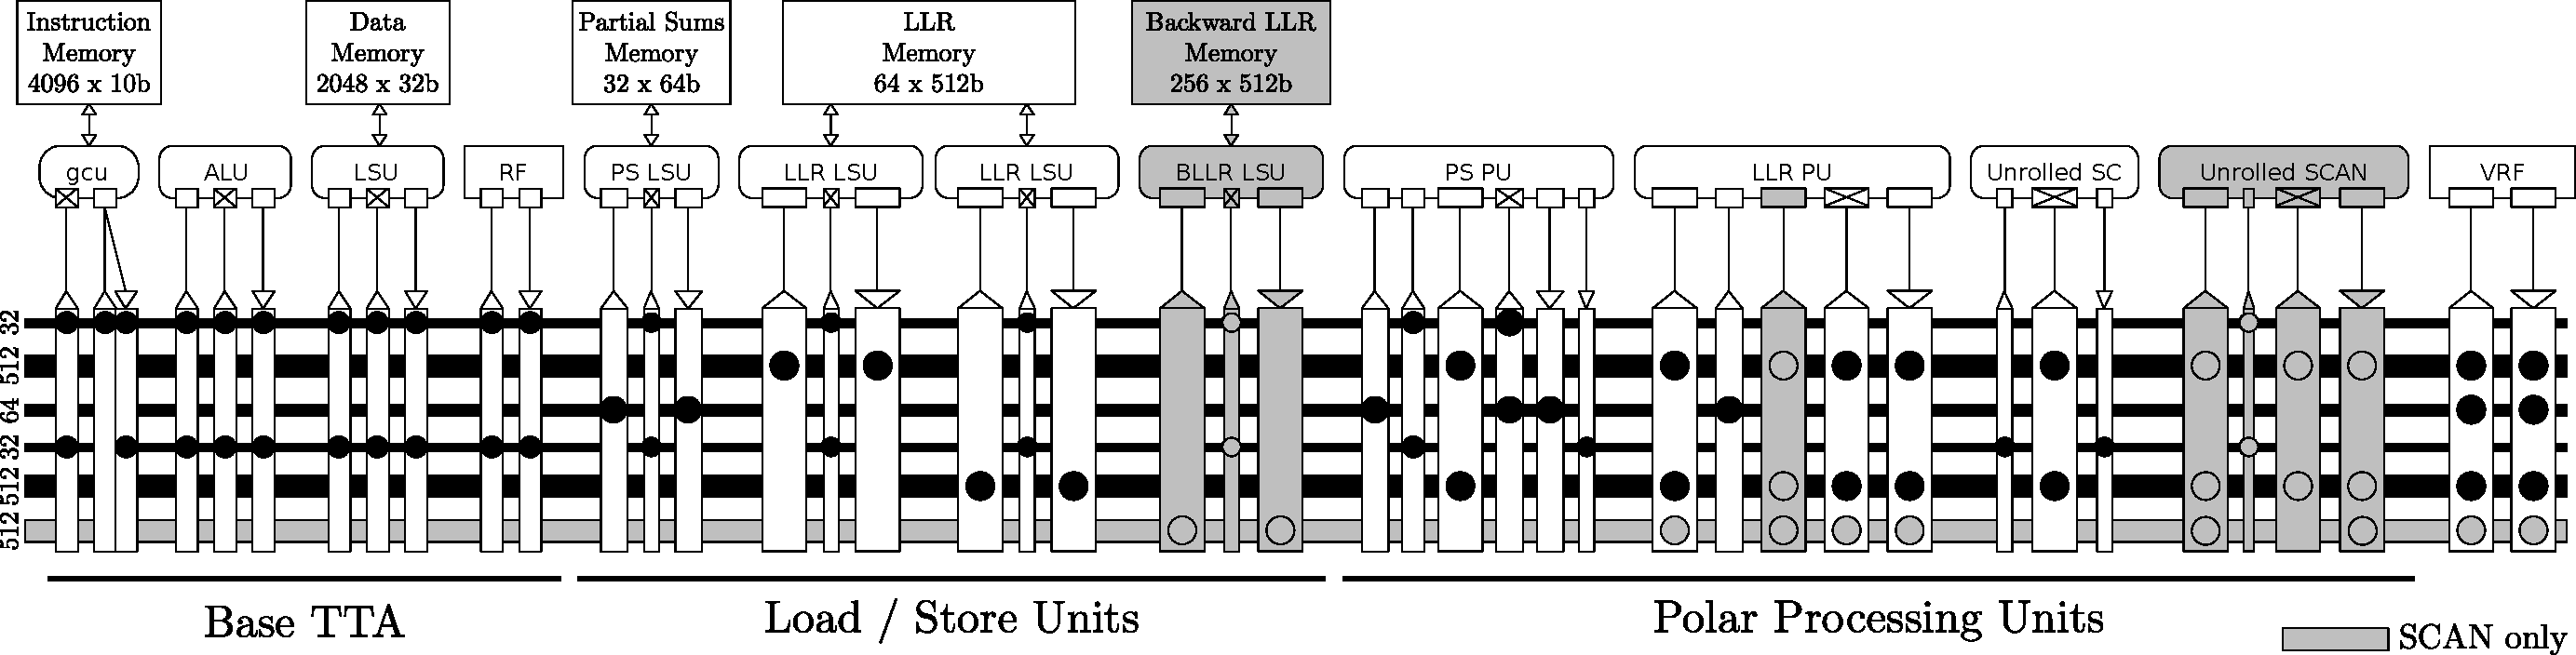
\includegraphics[width=\textwidth]{fig/prode}
	\caption{Transport Triggered Polar Decoder Architecture.}
	\label{fig:prode}
\end{figure*}

\begin{table}
  \centering
  \caption{Comparison of programmable processors running the SC decoding algorithm for R=0.5 polar codes}
  \label{tab:sw}
  {\small\resizebox{0.6\linewidth}{!}{
  \begin{tabular}{ccccc}
    \toprule
    Architecture & $N$ & \begin{tabular}{c}Latency\\{[$\mu$s]}\end{tabular} & \begin{tabular}{c}Throughput\\{[Mb/s]}\end{tabular} & \begin{tabular}{c}$E_b$\\{[nJ/bit]}\end{tabular} \\
    \cmidrule(lr){1-1}
    \cmidrule(lr){2-2}
    \cmidrule(lr){3-5}

    \multirow{2}{*}{\bf i7-3.3GHz}              & $1024$   & $2.0$  & $257$ & $41$ \\
                                                & $512$    & $1.2$  & $210$ & $49$ \\
    \multirow{2}{*}{\bf (GPP)}                  & $256$    & $0.7$  & $179$ & $59$ \\
                                                & $128$    & $0.4$  & $143$ & $73$ \\
    \midrule
    \multirow{2}{*}{\bf A57-1.1GHz}             & $1024$   & $10.7$ & $48$  & $17$ \\
                                                & $512$    & $5.3$  & $48$  & $17$ \\
    \multirow{2}{*}{\bf (GPP)}                  & $256$    & $2.8$  & $46$  & $17$ \\
                                                & $128$    & $1.6$  & $41$  & $20$ \\
    \midrule
    \multirow{2}{*}{\bf LX7-835MHz}             & $1024$   & $7.2$  & $71$  & $1.6$ \\
                                                & $512$    & $3.9$  & $66$  & $1.7$ \\
    \multirow{2}{*}{\bf (ASIP)}                 & $256$    & $1.9$  & $65$  & $1.7$ \\
                                                & $128$    & $1.0$  & $62$  & $1.8$ \\
    \midrule
    \multirow{2}{*}{\bf TTPD-800MHz}            & $1024$   & $1.4$  & $352$ & $0.14$   \\
                                                & $512$    & $0.8$  & $313$ & $0.15$   \\
    \multirow{2}{*}{\bf (ASIP)}                 & $256$    & $0.4$  & $304$ & $0.16$   \\
                                                & $128$    & $0.2$  & $284$ & $0.17$   \\
    \bottomrule
  \end{tabular}}}
\end{table}

\begin{table}[b]
  \centering
  \caption{ASIC implementations of dedicated SC decoders for a (1024,512) polar code}
  \label{tab:asic}
  {\small\resizebox{0.6\linewidth}{!}{

  \begin{tabular}{rcccc}
    \toprule
    & Proposed TTPD  & \cite{Giard2017} & \cite{mishra_successive_2012} & \cite{mishra_successive_2012}\parnote{{\footnotesize Scaling factors from 180nm to 28nm of \cite{mishra_successive_2012} are taken from \cite{Giard2017}.}} \\
    \cmidrule(lr){2-2}
    \cmidrule(lr){3-3}
    \cmidrule(lr){4-5}
    \textbf{Target}         &  28nm      & 28nm   & 180nm & 28nm  \\
    \textbf{Clock cycles}   &  1161      & 1833   & 1568  & 1568  \\
    \textbf{IT/P [Mb/s]}    &  352       & 94     & 49    & 436   \\
    \textbf{Freq [MHz]}     &  800       & 336    & 150   & 1335  \\
    \textbf{Power [mW]}     &  48        & 18     & 67    & 5     \\
    $\mathbf{E_b}$ [nJ/bit] &  0.14      & 0.19   & 1.4   & 0.011 \\
    \textbf{Area [mm$^2$]}  &  0.16      & 0.44   & 1.71  & 0.04  \\
    \textbf{Pruning}        &  R0 \& R1  & First R0  & None  & None  \\
    \bottomrule
  \end{tabular}}}
  \parnotes
\end{table}

\paragraph{Transport Triggered Polar Decoders} The proposed architecture, illustrated in Figure \ref{fig:prode}, builds upon a Base TTA and extends it with vector custom function units (FUs) to enable highly parallel processing. A vector size of $P=64$ was selected, allowing the FUs to process up to 64 data elements (LLRs or PSs) simultaneously. LLRs are represented as $Q=8$-bit values, ensuring negligible decoding performance loss. Core components of the architecture include parallel Load/Store Units (LSUs) for efficient memory access, Polar Processing Units (PPUs) that implement the specific $f$ and $g$ polar functions, and an unrolled SC decoder designed to accelerate the most sequential parts of polar decoding. A Vector Register File is included to buffer vector data and facilitate smooth data transfers between FUs.

The LSUs are tailored for high throughput, supporting the maximum polar code length of $N_\text{max}=1024$ as defined in the 5G standard \cite{ETSI2018}. PS memory is organized as 32x64 bits to allow parallel access to $P=64$ data, while LLR memory is mapped into a 64x512-bit RAM. The LSUs are optimized to reduce load/store latency from three to one clock cycle by removing internal registers, and they also support unaligned memory accesses without affecting the critical path, which remains in the 32-bit scalar ALU.

The PPUs, comprising the PS PU and LLR PU, act as SIMD units specialized for polar decoding, allowing multiple $f$ and $g$ operations to be performed in parallel. To further accelerate computation, unrolled subtree decoders are integrated as FUs for the lower stages of the decoding tree. These unrolled SC decoders can process 8 LLRs in 6 clock cycles, using a multi-cycle timing strategy instead of additional registers. This approach removes unnecessary hardware, keeps the critical path in the general-purpose ALU, and maintains full flexibility for varying frozen bit patterns. Overall, the architecture leverages vectorized FUs, efficient memory access, and unrolled subtree processing to achieve high-performance polar decoding while preserving the programmability and modularity of the Base TTA.

\paragraph{Results} A fine-grain comparison of polar decoders is challenging due to differences in technology, algorithms, pruning strategies, quantization, and frozen bit locations. Nevertheless, the Transport Triggered Polar Decoder (TT-SC), customized for SC decoding, demonstrates that TTA provides a natural compromise between programmable and dedicated architectures. Compared to previous work, the proposed TT-SC processor achieves significantly higher throughput and energy efficiency.

The TT-SC decoder was implemented using a 28 nm FD-SOI library, with memories realized in SRAM blocks. For a (1024, 512) polar code, it achieves a throughput of 352 Mb/s, which is 37\% higher than an Intel i7 CPU implementation, while consuming only 0.14 nJ/bit, two orders of magnitude lower than the general-purpose solution. Although more clock cycles are required than in dedicated architectures due to pipeline registration and more complete tree pruning, the TT-SC maintains comparable logic utilization and competitive hardware complexity while preserving programmability. Overall, the TT-SC processor illustrates that a TTA-based approach can deliver high-performance polar decoding while retaining flexibility.

\newpage


\section{Deep Learning on Embedded Targets}
\label{sec:deep_learning_embedded}

My arrival at IMT Atlantique in 2020 marked the beginning of my work on deep learning for embedded targets, with a particular focus on optimizing models for resource-constrained environments.

\subsection{Low-Cost Federated Learning}
Federated Learning (FL) is a promising approach for distributed machine learning, particularly suited for privacy-sensitive applications, such as military and medical domains, where client data cannot be shared or transferred to a cloud computing server. In standard FL, a server sends a model to a group of clients, who train it on their local data, then send their updated parameters back to the server for aggregation. This process aims to better guarantee user data privacy, as data never leaves the client device.

However, communication cost represents a major challenge in FL due to its intensive network usage. Client devices, such as smartphones or Internet of Things (IoT) nodes, have limited resources in terms of energy, computation, and memory. To overcome these hardware constraints, lightweight models and compression techniques such as pruning and quantization are commonly adopted in centralized paradigms.

In a first contribution, we proposed a method to insert the pruning technique as an additional step before communicating training results~\cite{grativol:hal-04251969,grativol:emse-04217775}. This approach aims to make messages sparser and thus reduce message size. More precisely, the method uses unstructured magnitude-based pruning, where weights with the smallest absolute values are replaced by zeros according to a predetermined pruning rate. This process is performed by the server and clients before transmitting a message, ensuring an equivalent pruning level throughout each communication round.

The results demonstrate that this method can compress messages by up to 50\% while incurring a precision loss of less than 1\%, outperforming state-of-the-art techniques. For example, with a 50\% pruning rate, message size is reduced to 23.0 MB, with an accuracy of 83.85±0.65\%, compared to 44.7 MB and 84.43±0.36\% for the full model without pruning. An increase in the number of local iterations per client during training contributes to a more robust model, allowing for sparser data communications while maintaining similar precision.

In a second contribution, we introduce FLoCoRA, a method that integrates LoRA techniques into the training of small vision models in a federated learning (FL) context~\cite{grativol:hal-04617632}. Unlike previous approaches focused on large models, FLoCoRA adopts an aggregation-agnostic strategy and keeps the base model frozen throughout training. Only the parameters of the much lighter LoRA adapters are updated and exchanged between clients. This design limits both data exchanges and memory usage, thanks to the absence of calculation and storage of the main model's gradients.

Key contributions include: the integration of LoRA adapters into the FL framework, with an implementation compatible with any FL optimization method, thus establishing a solid foundation for communication and memory reduction; a reduction in message sizes of up to 4.8 times with a precision loss of less than 1\% for a CIFAR-10 classification task using a ResNet-8; and the extension of the method with an affine quantization scheme, allowing for even higher compression rates, dividing the communication cost by 18.6 times, while maintaining a precision loss of less than 1\% on a ResNet-18 model.

Compared to conventional compression methods, FLoCoRA achieves less precision degradation for reduced message sizes. For example, for a pruning rate of 40\% (27.1 MB) with the magnitude pruning method, the precision is 85.20±0.20\%. In contrast, FLoCoRA with a rank of 64 and 8-bit quantization (2.4 MB) achieves 85.24±0.23\%, representing an 18.6-fold reduction in communication cost compared to the full FedAvg model (44.7 MB). The integration of affine quantization allowed for a 64-fold reduction in communication cost with an approximately 4\% precision loss.

This work demonstrates that LoRA, while commonly used for fine-tuning, can serve as a solid basis for communication savings in FL, paving the way for the deployment of Federated Learning on edge devices where communication is a bottleneck and computational power is limited.


\subsection{Compression by Pruning or Quantization and Embedded Deployment}

Another set of contributions focused on neural network pruning and was carried out as part of Hugo Tessier's thesis, in collaboration with Matthieu Arzel and Vincent Gripon from IMT Atlantique, thanks to CIFRE funding from the company Stellantis, with Thomas Hannagan and David Bertrand as supervisors.
A first notable contribution concerns the efficient pruning of neural networks through the targeted application of weight decay to a subset of weights. This method, named Selective Weight Decay (SWD) or Pénalisation Sélective des Pondérations (PSP), is described in articles~\cite{tessier:hal-03675138,tessier:hal-03695958}. Inspired by Lagrangian smoothing, SWD allows progressive and continuous pruning during training. It relies on adding a penalty term to the objective function, with a coefficient $a$ exponentially increasing between $a_{min}$ and $a_{max}$. This scheme ensures undisturbed initial training, followed by effective connection pruning when $a_{max}$ is sufficiently high.
SWD applies to both unstructured pruning (reducing low-norm weights to zero) and structured pruning (removing entire channels via the multiplicative coefficients of normalization layers).

The results show particular effectiveness for high pruning rates, where classical approaches significantly degrade performance. On datasets like CIFAR-10 and ImageNet ILSVRC2012, SWD outperforms reference methods. Its robustness and transferability are supported by an in-depth literature review. A high-impact blog post also popularized this approach\footnote{\url{https://towardsdatascience.com/neural-network-pruning-101-af816aaea61/}}.

However, pruning more complex models, such as those dedicated to semantic segmentation, presents specific challenges in achieving tangible gains on embedded targets, notably due to dimensional inconsistencies between layers. Solutions have been proposed to leverage global structured pruning while evaluating its real impact on energy consumption on embedded GPUs.
The proposed method solves these problems by first identifying all parts of the network that are disconnected when filters are removed, taking into account all architectural dependencies~\cite{tessier:hal-03706472}. It then automatically adapts addition operations to handle tensors of different dimensions, which ensures that all filters and kernels contribute to the network function, thus allowing a more reliable measurement of the actual pruning rate and the associated complexity of the pruned networks. In particular, additions at the end of each residual block in architectures like ResNet or HRNet require both input tensors to have the same dimensions, which can be resolved by replacing additions with a new "indexing-addition" operation.

Experiments conducted with this approach on NVIDIA Jetson AGX Xavier embedded GPUs demonstrated that global structured pruning can reduce energy consumption. However, it was found that smaller, unpruned networks, such as HRNet-32 and HRNet-18, are more energy-efficient than pruned networks, even with the same number of operations. This is attributed to the unconventional nature of the insertion operations (ScatterND) used to manage dimensions, which can harm the optimization of the rest of the network~\cite{tessier:hal-03767634,tessier:hal-03767636}. These results highlight the need for a more efficient implementation of the operators necessary to exploit pruning and to further explore the biases of pruning criteria, as they can lead to energy-suboptimal sparsity distributions.

In addition, other instances of performance improvement through pruning and quantization have been explored. An industrial project, carried out in collaboration with the company GoodFloow, allowed for the study of the interoperability of compression techniques (pruning, quantization, and coding) for the deployment of convolutional neural networks on microcontrollers with limited memory~\cite{younes:hal-03850858}. This work developed a methodology to optimize the trade-off between model accuracy and memory footprint, which is crucial for applications. Concurrently, research focused on the use of emerging memristor-based technologies for the development of binary neural networks~\cite{alhajali:hal-03659297}. These "in-memory computing" approaches aim to overcome the data bottleneck by performing calculations directly within memory, offering significant gains in speed and energy efficiency for binary neural networks, which are particularly well-suited for these technologies. Furthermore, developments of SIMD (Single Instruction Multiple Data) implementations for convolutional neural networks on general-purpose processors (GPP) were carried out in collaboration with the Canadian startup Deeplite~\cite{ganji:hal-04082069}. This project, called DeepGEMM, was based on the use of lookup tables (LUT) implemented using Intel AVX2 and Arm Neon instruction sets.

\subsection{Deep Learning on FPGA Targets}
Hugo Le Blevec's doctoral work focused on the co-design of deep neural networks and pipelined FPGA architectures for semantic segmentation in autonomous vehicles~\cite{leblevec:hal-04262138,leblevec:hal-04705594}. These systems require low latency and reduced consumption, making classic GPUs less suitable for embedded contexts. FPGAs offer a promising alternative due to their parallel processing and energy efficiency, although they pose challenges related to limited resources.

The thesis highlighted the often-underestimated impact of training routines. By optimizing these on a lightweight model like ENet, gains of over 12\% on Cityscapes and 26\% on CamVid were obtained. This demonstrates that careful training allows simple architectures to compete with more complex models.
The ENet architecture was then adapted for efficient FPGA mapping, relying on the open-source FINN framework. Notable contributions include the addition of streamlining transformations and the integration of transposed convolutions, essential for segmentation. The final model, P-ENet, achieves 70.3\% mIoU in INT4, with 4.2 ms latency and 226 FPS on Cityscapes. It outperforms existing FPGA implementations and proves to be 1.15 times more energy-efficient than an NVIDIA Jetson AGX Xavier. This work is not currently presented in the manuscript but is under submission to ACM TRETS.

In parallel, the PEFSL (Pipeline for Embedded Few-Shot Learning) project, originating from a student project I supervised, winner of the 2023 OpenHardware AMD Xilinx competition\footnote{https://www.openhw.eu/2023-results-gallery}, tackled few-shot learning on FPGA-SoC. The developed flow, based on Tensil, covers the entire training, design chain, and deployment on a PYNQ-Z1 board. The demonstrator achieves a latency of 30 ms for a consumption of 6.2 W on MiniImageNet~\cite{grativol:hal-04559365}.

This work led to a collaboration with Tohoku University and Professor Naoya Onizawa, materialized by reciprocal visits and two publications~\cite{kanda:hal-04984380,kanda:hal-04984381}. These articles aim to ensure precision consistency throughout the design flow by applying fixed-point quantization via Brevitas, with QAT and PTQ methods. They show that near floating-point precision can be achieved with only 5 to 6 bits for both integer and fractional parts. These models were then integrated into the FINN suite within PEFSL.

\chapter{Research Perspectives}
% \minitoc
% \vspace{1cm}
\clearpage
\section{New Methods and Architectures for Channel Codes}
\subsection{Interest in Short Codes, Relevance of Polar Codes}

Currently, software implementations of error-correcting codes are highly sought after. They offer great flexibility and reduce development and deployment costs compared to dedicated hardware solutions. I am currently planning to collaborate with ETS Montreal to implement the \textit{Generalized Restart Mechanism} (GRM) algorithm \cite{Sagitov2025}. GRM reduces the average execution time of decoders by skipping identical calculations between decoding attempts. This technique, applicable to Successive-Cancellation Flip (SCF) and Fast-SCF, decreases execution time by 25\% to 60\% without degrading error correction, with only 4\% additional memory. For its implementation, software optimization techniques such as unrolling and vectorization will be used. Preliminary results show that gains in throughput and especially in maximum latency, a weak point of the Adaptive SCL algorithm, are very significant.

These developments could extend to quantum polar codes. The Successive Cancellation List (SCL) decoder is adaptable to quantum polar codes, offering high performance and low complexity \cite{Gong2024}. A new construction of quantum polar codes based on weight polarization (PW) eliminates the need for entanglement assistance. The SCL-C decoder is currently based on the list algorithm. It would be possible to adapt it to GRM-SCF, thereby greatly reducing complexity, down to a complete software implementation. We also have collaboration opportunities on the subject of constructing polar codes adapted to SCF decoding using deep learning, similar to work I presented at the ISTC 2023 conference~\cite{leonardon:hal-03291030}.

\subsection{RISC-V Architectures for Channel Code Decoding}

For the embedded domain, there are very good reasons to explore RISC-V architectures, an open and free instruction set architecture (ISA), which contrasts with proprietary architectures like ARM or x86. This openness allows chip designers and system developers to customize the architecture for specific applications without paying licensing fees, thus offering increased flexibility and innovation.
One of the major advantages of RISC-V for embedded systems is its modularity. It allows for the addition of custom extensions, which is ideal for specialized workloads, such as error-correcting code decoding. This means it is possible to design a processor with specific instructions that directly accelerate decoding operations, leading to better performance and energy efficiency than what would be possible with a generic architecture.

Furthermore, the RISC-V ecosystem is rapidly growing, with increasing support from industry and academia. This fosters the development of tools, software, and hardware that facilitate design and deployment. The open-source aspect of RISC-V also encourages transparency and security, crucial elements for critical embedded systems.

With this in mind, I plan to collaborate with Adrien Cassagne from LIP6 (for software acceleration aspects) and Camille Leroux (hardware acceleration) from Bordeaux INP to set up a collaborative ANR (PRC) focused on the design of specialized RISC-V architectures for error-correcting code decoding. This initiative would aim to fully exploit the customization potential of RISC-V to create highly optimized and high-performance embedded solutions.

\section{Network Specialization for Embedded Targets}

As previously shown, numerous contributions have been made in the field of deep learning on embedded targets, particularly concerning model compression and their deployment on specific hardware architectures. This work motivates new developments. On the one hand, their application in specific domains, notably their use in the context of signal jamming in launchers or the processing of EEG signals. On the other hand, the need to take a step back and find more systematic approaches for designing deep learning models adapted to the constraints of embedded targets, particularly by using co-design techniques between models and hardware architectures based on NAS (Neural Architecture Search).

\subsection{Application of Deep Learning for GNSS Denoising in a Spatial Context}
Following several works carried out within the framework of previous research contracts with the company Arkane, a central issue emerged: the persistent vulnerability of Global Navigation Satellite Systems (GNSS) to interference, jamming, and other forms of signal degradation. These observations led to the definition of a CIFRE thesis project whose objective is to propose innovative solutions to improve the resilience of these systems, particularly in critical contexts such as space environments or embedded applications with strong constraints.

The project is particularly interested in Controlled Reception Pattern Antennas (CRPA), capable of spatially processing signals to mitigate disturbances. However, classical beamforming methods, although theoretically powerful, remain computationally expensive and poorly suited to embedded constraints. To overcome these limitations, the proposed work explores the integration of Deep Learning, and notably convolutional models, to simplify and accelerate spatiotemporal processing performed by these antennas.

One of the major challenges of the project lies in adapting these models to constrained hardware platforms, such as FPGAs, often used in embedded systems for their low energy consumption, reconfiguration capabilities, space qualification, and supply reliability. It will therefore be necessary to design neural network architectures that are efficient, compact, and interpretable, allowing real-time execution without compromising the quality of positioning, synchronization, or estimated speed. Particular efforts will also be devoted to model quantization, complexity reduction, and optimization of their deployment on the target hardware.

The adopted approach will be resolutely interdisciplinary, relying on continuous exchanges between the company and another research team involved from Télecom Paris (Comelec). The project plans an alternation between algorithmic design phases, prototyping, hardware implementation, and experimental validation. Tests will be conducted both in simulation and on real test benches, in order to rigorously evaluate the robustness and performance of the proposed solutions in representative environments.

Beyond the expected scientific advances, this work also aims to produce concrete and valuable results, whether in the form of embedded demonstrators, publications, or patent filings. One of the envisioned outlets concerns the improvement of autonomous navigation capabilities on board space launchers, an application domain already explored in previous works and for which technological transfer prospects are promising.

\subsection{Attention Layers on Microcontroller Targets for EEG Data Processing}

A project currently being structured within the BRAIN team focuses on the application of Transformers to real-time processing of electroencephalographic (EEG) signals in embedded environments. Transformer-type architectures have recently shown very good performance for analyzing EEG data, particularly due to their ability to capture long-range dependencies in multichannel signals~\cite{tegon2025}. This methodological orientation is increasingly present in the literature but remains little explored in the context of embedded deployment.

A notable specificity of EEG work is the use of long time sequences, often necessary to capture brain rhythms or discrete events. This poses a major challenge for embedded systems, as the complexity of Transformers grows rapidly with sequence length. In contrast, unlike what is observed in language or image processing, EEG models use relatively compact architectures, which makes their execution on microcontrollers feasible, provided targeted optimization work.

The project's objective is to design a real-time embedded processing demonstrator based on Transformers optimized for EEG. This involves rigorous hardware-software co-design: memory footprint control, operation vectorization to take advantage of microcontroller parallel architectures, and adaptation of model layers to hardware constraints. A collaboration is planned with Giulia Lioi, to ensure the relevance of the methods and tasks envisioned and to anchor the project in concrete use cases. This work could lead to lightweight, autonomous devices capable of localized EEG processing, with potential applications in neurotechnology, portable diagnostics, or brain-machine interfaces.

\subsection{Co-design of Neural Networks and Embedded Hardware Architectures}

Finally, a possible improvement to my current work lies in the fact that architecture design is performed manually. Neural Architecture Search (NAS) is a well-known and frequently cited approach for automating the design of neural network architectures. However, this field is often perceived as disconnected from practical realities, producing architectures that are not always optimized for real-world constraints.

Zero-cost proxies (ZCPs), which enable low-cost NAS by avoiding full model training, present a fundamental limitation~\cite{lymanson:hal-04576139}. Although they show a strong correlation with model performance across the entire search space, this correlation drastically decreases when focusing on the best architectures. ZCPs tend to be biased towards architectures with a large number of parameters, which reduces their discriminatory power for high-performance models. This weakness is particularly notable when the search space is reduced to the top 1\% of architectures, where the correlation between ZCPs and actual performance drops significantly.

To overcome this problem, my objective is to develop more pragmatic techniques to automatically design lightweight neural network architectures, whether Transformers or CNNs. Preliminary work in this direction has already been carried out. We are currently focusing on sampling techniques on supernets, guided by zero-shot metrics, to automate this design more efficiently and adapted to implementation constraints. The number of model parameters is considered a simple but universal discriminant metric to constrain the search space, thus targeting regions more suitable for ZCP-guided exploration. This approach aims to improve the quality of discovered architectures, especially for ZCPs that struggle to find high-performing regions of the space on their own, and allows controlling the size of sampled models, thus avoiding over-parameterizing architectures.

Similarly, an effective technique for designing neural network models by NAS is the Supernet paradigm. This involves training a neural network model encompassing a wide variety of possible architectures, thereby enabling the discovery of high-performing models without having to train each architecture individually. One of the problems is how to perform the training so that, in the end, sub-networks are capable of functioning autonomously. In most methods, a selection of sub-networks to be agglomerated with the loss is performed, but this selection is done randomly. We could instead focus on architectures that are known to be high-performing, for example by using zero-cost proxies. Or, by using expert models on the suitability of sub-networks for given hardware architectures. The Stream tool developed by the MICAS team at the University of Louvain allows for this modeling, for example~\cite{symons2022}. We have contacted this team, and Jérémy Morlier, a doctoral student as part of my JCJC ProPruNN project, has begun working on integrating Stream into the search for sub-networks for specific hardware architectures. A mobility period in autumn 2025 is planned to deepen this collaboration and explore the possibilities offered by Stream in the context of searching for sub-networks adapted to hardware constraints.

\appendix

\chapter{Curriculum Vitae}
\section{Summary of Professional Career and Academic Activities}




% Inclure pdf main-french.pdf
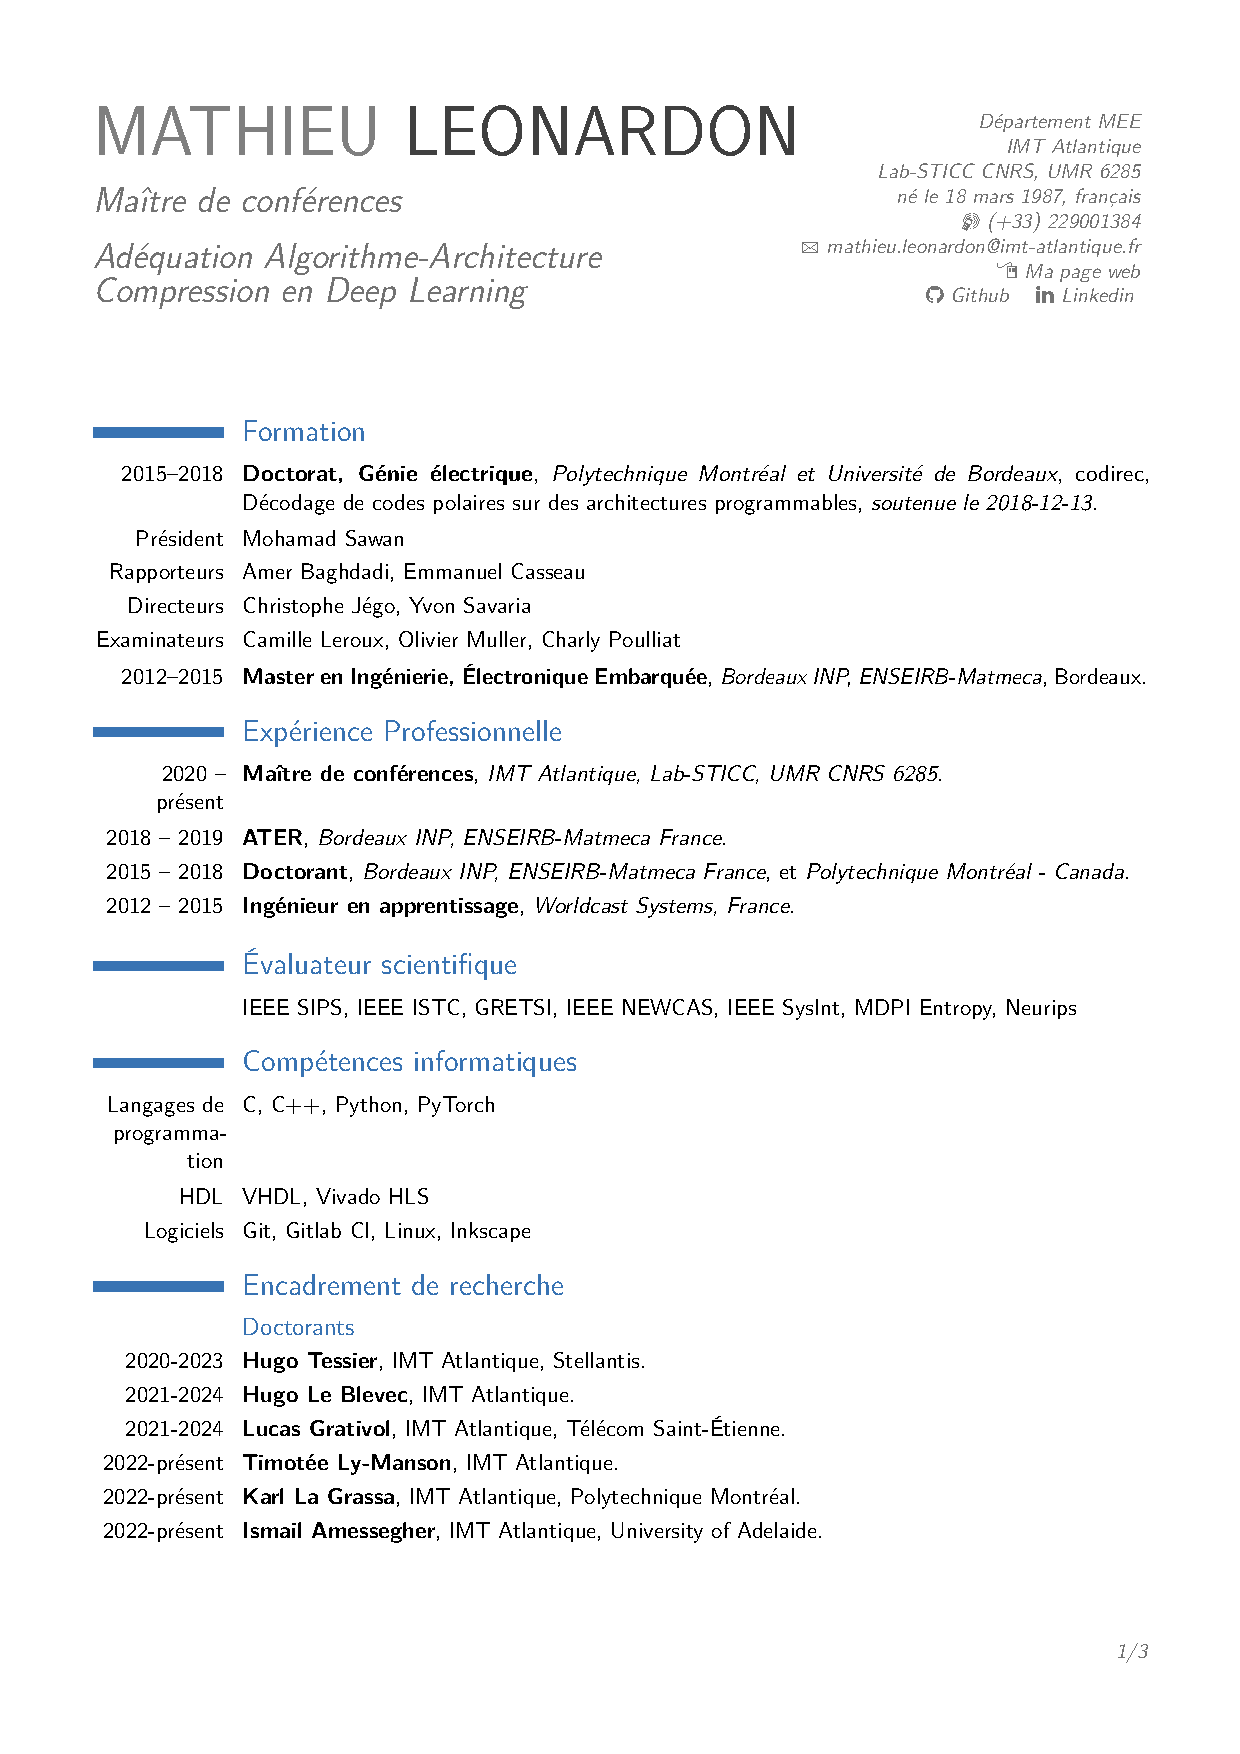
\includepdf[
  pages=-,
  pagecommand={\thispagestyle{includepdfstyle}}
]{main_french.pdf}
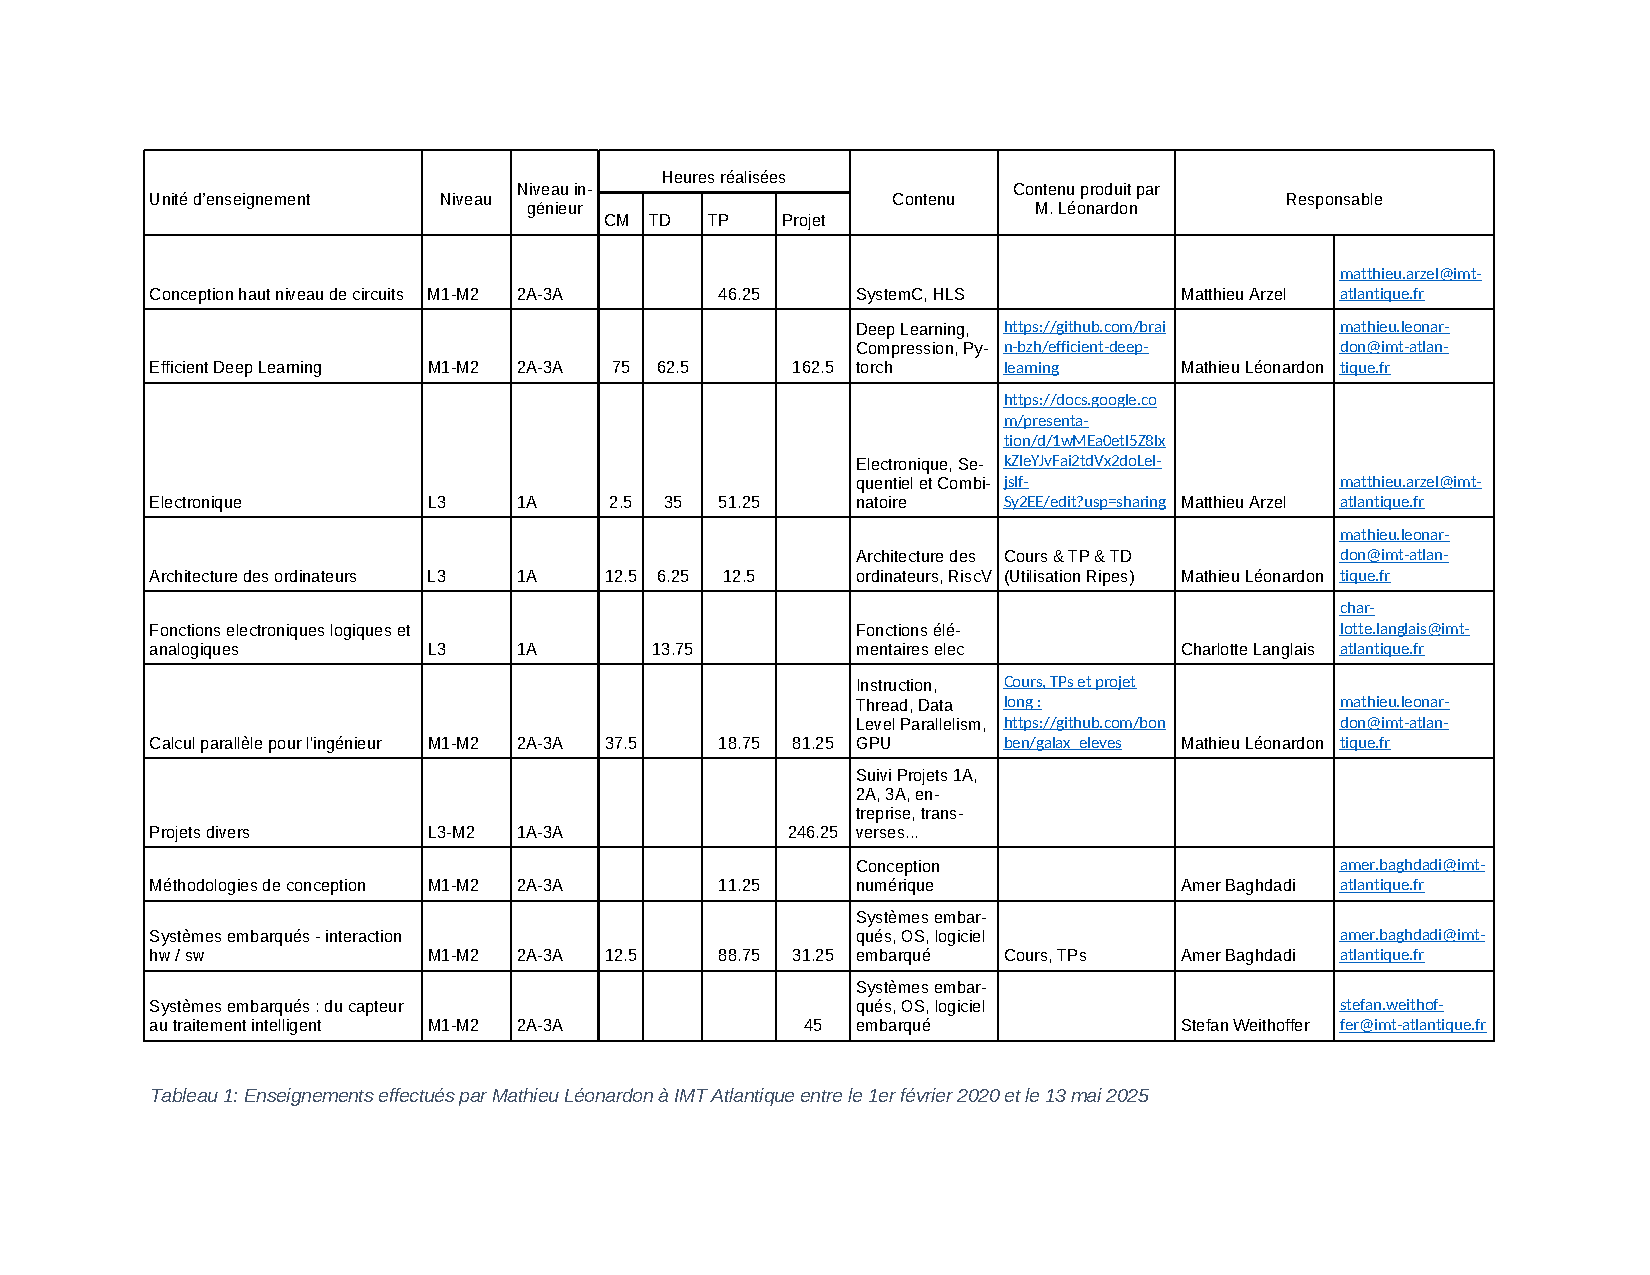
\includepdf[
  pages=-,
  pagecommand={\section{Teaching Activities}\thispagestyle{includepdfstyle}}
]{enseignements.pdf}

\section{Spotlight on two courses}
\label{sec:spotlight_courses}

\section{Publications}
\subsection{PhD Thesis}
\printbibliography[keyword={MANUSCRIPT}, heading=none]
\subsection{Publications in International Journals}
\printbibliography[keyword={JOURNAL}, heading=none]
\subsection{Publications in International Conferences with Proceedings}
\printbibliography[keyword={CONFERENCE}, heading=none]
\subsection{Publications in National Conferences with Proceedings}
\printbibliography[keyword={NATIONAL}, heading=none]
\subsection{Communications without Proceedings}
\printbibliography[keyword={WORKSHOP}, heading=none]


\pagebreak
\section{Summary of Supervision Activities}
\label{sec:encadrement}

\subsection{Doctoral Student Supervision}
Theses defended:
\begin{itemize}
    \item Hugo Tessier, defended on 09/02/2023
    \begin{itemize}
      \item 25\% - Participation in Hugo's thesis covered all research work, with a particular focus on deployment on embedded targets.
    \end{itemize}
    \item Lucas Grativol Ribeiro, defended on 05/12/2024
    \begin{itemize}
      \item 25\% - Participation in the design of this Futur et Ruptures thesis with colleagues from Telecom and Mines Saint Etienne. Provided expertise on the choice of learning models and the application of compression techniques.
    \end{itemize}
    \item Hugo Le Blevec, defended on 06/12/2024
    \begin{itemize}
      \item 50\% - Co-supervision of Hugo Le Blevec's thesis. Participation in all research work, particularly initiating collaborations with the AMD team in Dublin (Thomas Preusser).
    \end{itemize}
\end{itemize}
Theses in progress:
\begin{itemize}
    \item Timotée Ly-Manson, defense scheduled for December 2025
    \begin{itemize}
      \item 50\% - Co-supervision of Timotée Ly-Manson's thesis, funded by my research contracts and subject designed with him. Collaboration established with the Sony Stuttgart team, particularly Lukas Mauch.
    \end{itemize}
    \item Ismail Amessegher, defense scheduled for December 2025
    \begin{itemize}
      \item 33\% - Co-supervision of Ismail Amessegher's thesis, with involvement in the deployment of object detection models on FPGA.
    \end{itemize}
    \item Jérémy Morlier, defense scheduled for December 2026
    \begin{itemize}
      \item 50\% - Co-supervision of Jérémy Morlier's thesis, funded by the JCJC ProPruNN project.
    \end{itemize}
    \item Elise Lagarde, since January 2025
    \begin{itemize}
      \item 50\% - Initiated this CIFRE thesis in collaboration with Arkane and Telecom Paris, following a previous research contract.
    \end{itemize}
\end{itemize}

\subsection{Master's Internship Supervision}
\begin{itemize}
    \item Hugo Kermabon, May to August 2020
    \item Hugo Le Blevec, April to October 2020
    \item Jérémy Morlier, June to July 2021
    \item Lubin Gauthier, July to September 2023
    \item Pedro Figueireido, May to August 2025
    \item Mohammed El Houcine Ayoubi, April to August 2025
\end{itemize}
% \small % Réduit la taille de la police pour tout le tableau
% \begin{longtable}{|p{0.25\linewidth}|p{0.13\linewidth}|c|p{0.18\linewidth}|c|p{0.15\linewidth}|}
% \caption{Activités d'enseignement} \label{tab:activites_enseignement} \\
% \hline
% \textbf{Nom de l'enseignement} & \textbf{Membre ou Lead} & \textbf{HETD} & \textbf{\'Etablissement} & \textbf{Ann\'ee scolaire} & \textbf{Niveau} \\
% \hline
% \endfirsthead
% \hline
% \textbf{Nom de l'enseignement} & \textbf{Membre ou Lead} & \textbf{HETD} & \textbf{\'Etablissement} & \textbf{Ann\'ee scolaire} & \textbf{Niveau} \\
% \hline
% \endhead
% \hline
% \endfoot
% \hline
% \endlastfoot
% Projet de conception en \'electronique & Lead & 50.00 & ENSEIRB-MATMECA & 2015-2020 & L3\\
% Architecture reconfigurable & Lead & 20.00 & ENSEIRB-MATMECA & 2015-2020 & M1\\
% \'Electronique Num\'erique & Lead & 25.00 & ENSEIRB-MATMECA & 2015-2020 & L3\\
% Logique combinatoire et logique s\'equentielle & Membre & 32.00 & ENSEIRB-MATMECA & 2015-2020 & L3\\
% Projet micro-processeur & Membre & 36.00 & ENSEIRB-MATMECA & 2015-2020 & L3\\
% Architecture des ordinateurs & Membre & 16.00 & ENSEIRB-MATMECA & 2015-2020 & M1\\
% Projet micro-informatique & Membre & 42.00 & ENSEIRB-MATMECA & 2015-2020 & M1\\
% Programmation objet. Langage C++ & Membre & 15.00 & ENSEIRB-MATMECA & 2015-2020 & M1\\
% Conception haut niveau de circuits & Membre & 46.25 & IMT Atlantique & 2020-2025 & M1-M2\\
% Efficient Deep Learning & Lead & 300.00 & IMT Atlantique & 2020-2025 & M1-M2\\
% Electronique & Membre & 88.75 & IMT Atlantique & 2020-2025 & L3\\
% Architecture des ordinateurs & Lead & 31.25 & IMT Atlantique & 2020-2025 & L3\\
% Fonctions electroniques logiques et analogiques & Membre & 13.75 & IMT Atlantique & 2020-2025 & L3\\
% Calcul parall\'ele pour l'ing\'enieur & Lead & 137.50 & IMT Atlantique & 2020-2025 & M1-M2\\
% Projets divers & Membre & 246.25 & IMT Atlantique & 2020-2025 & L3-M2\\
% M\'ethodologies de conception & Membre & 11.25 & IMT Atlantique & 2020-2025 & M1-M2\\
% Syst\'emes embarqu\'es - interaction hw \textbackslash{} sw & Membre & 132.50 & IMT Atlantique & 2020-2025 & M1-M2\\
% Syst\'emes embarqu\'es : du capteur au traitement intelligent & Membre & 45.00 & IMT Atlantique & 2020-2025 & M1-M2\\
% \end{longtable}
\begin{landscape}
\section{Research Funding}
\label{sec:financement}

\subsection{Public Funding}
{\small
\begin{longtable}{|c|l|p{3cm}|p{1.cm}|p{1.5cm}|p{6.5cm}|}
\caption{Public Funding} \label{tab:financements_publics} \\
\hline
\textbf{Year} & \textbf{Short Title} & \textbf{Organization} & \textbf{Role} & \textbf{Amount (k€)} & \textbf{Details}\\
\hline
\endfirsthead
\endfoot
\hline
\endlastfoot
2023-2027 & Autonomous Pack & ADEME Logistique 4.0& PI & 260  & Principal investigator of the project. Expertise on embedding neural networks on accelerometer data on microcontrollers\\
2024-2026 & GNSS Anti-Jamming w/ CRPA \& CNN/TCN & R\'egion Bretagne & co-PI & 140  & Participation in the project supervising a post-doctoral researcher on porting embedded learning processing to FPGA\\
2023-2026 & ProPruNN: Pruning Neural Networks & ANR JCJC& PI & 250  & Principal investigator of my JCJC project on the co-design of deep learning models and hardware architectures\\
2023-2026 & Vortex: Drone Swarms for Exploration & ANR TSIA & co-PI & 200  & Supervision of a doctoral student, Ismail, on the implementation of object detection algorithms on event data\\
2024-2025 & Deep-Learning-FPGA-Eco-conception & CNES & PI & 5  & Responsible for a training course on neural network compression for the company Arkane\\
2021-2025 & GoodFloow & ADEME Perfecto & PI & 70  & Principal investigator of the project for IMT Atlantique, by supervising a post-doctoral researcher, Hamoud Younes\\
2022-2024 & Leasard: Low Energy DNN for Drones & Labex CominLabs & co-PI & 120  & Supervision of a doctoral student, Ismail, on the implementation of object detection algorithms on event data\\
2022-2024 & FLCNNFPGA: Federated Learning & CNRS GDR ISIS & PI & 7  & Funding for a master's internship and equipment as part of Lucas Grativol's thesis\\
2021-2024 & FLCNNFPGA: Federated Learning \& FPGA & IMT Futur \& Ruptures & co-PI & 120 & Supervision of Lucas Grativol \\
\end{longtable}
}

\subsection{Private Funding}
{\small
\begin{longtable}{|c|l|p{3cm}|p{1cm}|p{1.5cm}|p{6.5cm}|}
\caption{Private Funding} \label{tab:financements_prives} \\
\hline
\textbf{Year} & \textbf{Short Title} & \textbf{Organization} & \textbf{Role} & \textbf{Amount (k€)} & \textbf{Details} \\
\hline
\endhead
\hline
\endfoot
\hline
\endlastfoot
2025-2028 & GNSS Anti-Jamming Opt. (CIFRE) & Arkane & co-PI & pvt & Initiator of Elise Lagarde's CIFRE thesis, responsible for the FPGA target implementation part\\
2023-2025 & Few-Shot NAS in Metric-Driven Fmwk & Sony & co-PI & 180k€ & Project with Sony on many topics including few-shot learning and LLMs. For my part, I participated in the writing of an article on NAS\\
2024-2025 & Embedded DL for Seg. \& LLMs & Schneider Electric & PI & 40k€ & Principal investigator of this project, which focused on the integration of semantic segmentation networks on embedded targets on the one hand, and the implementation of RAG (retrieval-augmented generation) on embedded targets on the other.\\
2020-2023 & CNN Pruning for Embedded Vision (CIFRE) & Stellantis & co-PI & pvt & Participated in the supervision of Hugo Tessier upon my arrival at IMT Atlantique \\
2022 & DeepGEMM: Low-Precision Inference & Deeplite & PI & 60k€ & Principal investigator and lead developer of a quantized neural network implementation on embedded targets using LUTs and SIMD instructions.\\
\end{longtable}
}
\end{landscape}


\section{References}
\printbibliography[keyword={REFERENCE}, heading=none]

\end{document}